\documentclass[8pt]{beamer}\usepackage[]{graphicx}\usepackage[]{color}

\documentclass{article}
\usepackage{fancyhdr}


\pagestyle{fancy}
\fancyhf{}
\rhead{Ryan Giordano}
\lhead{Research Statement}
\rfoot{Page \thepage}

\usepackage{tabularx}

% \usepackage{fancyhdr}
% \pagestyle{fancy}

% \fancyfoot{}
% \fancyfoot[C]{Rough draft---do not distribute}

\usepackage{etoolbox}


\usepackage{microtype}
\usepackage{graphicx}
\usepackage{subfigure}
\usepackage{booktabs} % for professional tables
\usepackage{xcolor}
\usepackage[hidelinks=True]{hyperref}
\usepackage{xargs}[2008/03/08]

% Documentation
% http://ftp.math.purdue.edu/mirrors/ctan.org/macros/latex/contrib/refstyle/refstyle.pdf
\usepackage{refstyle}
\usepackage{varioref} % Use refstyle instead of varioref directly.

\usepackage{amsmath}
\usepackage{amssymb}
\usepackage{amsfonts}
\usepackage{amsthm}
\usepackage{mathrsfs} % For mathscr
\usepackage{mathtools}

\usepackage[authoryear]{natbib}
\bibliographystyle{apalike}

\usepackage{geometry}
\geometry{margin=1.5in}


\algblock{Inputs}{EndInputs}
\algnotext{EndInputs}

\algblock{Postprocessing}{EndPostprocessing}
\algnotext{EndPostprocessing}

\newtheorem{assu}{Assumption}
\crefname{assu}{assumption}{assumptions}

\newtheorem{lem}[theorem]{Lemma}
\crefname{lem}{lemma}{lemmas}

\newtheorem{ex}{Example}
\crefname{ex}{example}{examples}

\def\red#1{\textcolor{red}{#1}}
\def\blue#1{\textcolor{blue}{#1}}
\def\green#1{\textcolor{violet}{#1}}

\def\undernote#1#2{\underbrace{#1}_{\mathclap{\substack{#2}}}}
\def\overnote#1#2{\overbrace{#1}^{\mathclap{\substack{#2}}}}

\newcommand{\iid}{\overset{iid}{\sim}}

\newcommand{\dataset}{{\cal D}}
\newcommand{\fracpartial}[2]{\frac{\partial #1}{\partial  #2}}
\newcommand{\fracat}[3]{\left. \frac{#1}{#2} \right|_{#3}}
\newcommand{\trans}{\intercal}
\newcommand{\const}{C}
\newcommand{\diag}[1]{\mathrm{Diag}\left(#1\right)}
\newcommand{\grad}[2]{\nabla_{#1} \left. #2 \right.}
\newcommand{\hess}[2]{\nabla^2_{#1} \left. #2 \right.}
\newcommand{\gradat}[3]{\nabla_{#1} \left. #2 \right|_{#3}}
\newcommand{\norm}[1]{\left\Vert #1\right\Vert}
\newcommand{\abs}[1]{\left| #1\right|}
\newcommand{\normp}[1]{\left\Vert #1\right\Vert_*}
\newcommand{\trace}[1]{\mathrm{Tr}\left(#1\right)}
\newcommand{\oned}[1][\thetadim]{1_{#1}} % Vector of ones
\newcommand{\zerod}[1][2\thetadim]{0_{#1}} % Vector of zeros
\newcommand{\ident}[1][\thetadim]{I_{#1}} % Identity matrix
\newcommand{\dequal}{\stackrel{d}{=}}


\newcommand{\y}{y}  % data
\newcommand{\z}{z}  % Reparameterization trick variable
\newcommand{\Z}{\mathcal{Z}_{\znum}}  % Set of \z
\newcommand{\znum}{N} % Number of elements of \Z
\newcommand{\Zindep}{\tilde{\mathcal{Z}}}  % Set of \z
\newcommand{\p}{\mathcal{P}} % posterior and model probability
\newcommand{\q}{\mathcal{Q}} % vb approximation
\newcommand{\gfull}{\mathcal{G}} % Grad of exact KL
\newcommand{\g}{\hat{\gfull}} % Grad of MC KL
\newcommand{\hfull}{\mathcal{H}} % Hess of exact KL
\newcommand{\h}{\hat{\hfull}} % Hess of MC KL
\newcommand{\scorecov}{\hat{\Sigma}_{s}} % Estimated score covariance
\newcommand{\fun}{f} % Function of interest
\newcommand{\etahat}{\hat{\eta}}
\newcommand{\etatil}{\tilde{\eta}}
%\newcommand{\etastar}{\stackrel{*}{\eta}} % Superscripts are too high
%\newcommand{\etastar}{\eta^{*}} % Double superscript
\newcommand{\etastar}{\accentset{*}{\eta}}
\newcommand{\ghat}{\hat{g}} % MC estimate of model grad
\newcommand{\hhat}{\hat{h}} % MC estimate of model hessian


\newcommand{\qoi}[1]{\phi\left(#1\right)}
\newcommand{\qoigrad}[1]{\nabla_{\eta} \phi\left(#1\right)}
\def\normal#1#2{\mathcal{N}\left(#1 \vert #2\right)}
\def\wishart#1#2{\mathcal{W}\left(#1 \vert #2\right)}
\def\normz{\mathcal{N}_{\mathrm{std}}\left(\z\right)}
\newcommand{\post}{\p(\theta \vert \y)}
\newcommand{\logjoint}{\log \p(\theta, \y)}
\newcommand{\logjointgrad}{\nabla_{\theta} \log \p(\theta, \y)}
\newcommand{\logjointhess}{\nabla^2_{\theta} \log \p(\theta, \y)}
\newcommand{\etaopt}{\hat{\eta}}
\newcommand{\etaoptd}{\hat{\eta}_{D}}
\newcommand{\etaopts}{\hat{\eta}_{S}}

% https://stackoverflow.com/questions/1812214/latex-optional-arguments
\newcommand{\etamu}[1][]{\mu_{#1}}
\newcommand{\etamuhat}[1][]{\hat{\mu}_{#1}}
\newcommand{\etamustar}[1][]{\accentset{*}{\mu}_{#1}}

\newcommand{\etasigma}[1][]{\sigma_{#1}}
\newcommand{\etasigmahat}[1][]{\hat{\sigma}_{#1}}
\newcommand{\etasigmastar}[1][]{\accentset{*}{\sigma}_{#1}}

\newcommand{\etaxi}[1][]{\xi_{#1}}
\newcommand{\etaxihat}[1][]{\hat{\xi}_{#1}}
\newcommand{\etar}[1][]{{R_{#1}}}

\newcommand{\qdom}{\Omega_{\q}}
\newcommand{\thetadom}{\mathbb{R}^\thetadim}
\newcommand{\rdom}[1]{\mathbb{R}^{#1}}
\newcommand{\etadom}{\mathbb{R}^\etadim}

\newcommand{\thetadim}{{D_{\theta}}}
\newcommand{\etadim}{{D_{\eta}}}
\newcommand{\lambdadim}{{D_{\lambda}}}
\newcommand{\gammadim}{{D_{\gamma}}}

\def\expect#1#2{\underset{#1}{\mathbb{E}}\left[#2\right]}
\newcommand{\meanz}{\frac{1}{\znum} \sum_{n=1}^{\znum}}
\def\sumn{\sum_{n=1}^{N}}
\def\meann{\frac{1}{N}\sumn}
\def\sump{\sum_{p=1}^{P}}
\def\sumd{\sum_{d=1}^{\thetadim}}
\def\meann{\frac{1}{N}\sumn}
\def\expecthat#1#2{\underset{#1}{\widehat{\mathbb{E}}}\left[#2\right]}
\def\var#1#2{\underset{#1}{\mathrm{Var}}\left(#2\right)}
\def\lrcovfull#1#2{\underset{#1}{\mathrm{LRCov}}\left(#2\right)}
\def\lrcov#1#2{\underset{#1}{\widehat{\mathrm{LRCov}}}\left(#2\right)}
\def\lrvar#1#2{\underset{#1}{\mathrm{LRVar}}\left(#2\right)}
\def\cov#1#2{\underset{#1}{\mathrm{Cov}}\left(#2\right)}
\def\kl#1#2{\mathrm{KL}\left(#1 || #2\right)}
\def\klfullobj#1{\mathrm{KL}_{\mathrm{VI}}\left(#1\right)}
\def\klobj#1{\widehat{\mathrm{KL}}_{\mathrm{VI}}\left(#1\right)}
\def\expectpost#1{\expect{\post}{#1}}

% High dimensional normals notation
\def\zbar{\bar{z}}
\def\zzbar{\overline{zz^\trans}}
\def\sigmat{S}
\def\zcov{\hat{\Sigma}_{z}}


\DeclareMathOperator*{\argmax}{\mathrm{argmax}}
\DeclareMathOperator*{\argmin}{\mathrm{argmin}}
\DeclareMathOperator*{\esssup}{\mathrm{esssup}}
\DeclareMathOperator*{\essinf}{\mathrm{essinf}}
\DeclareMathOperator*{\argsup}{\mathrm{argsup}}
\DeclareMathOperator*{\arginf}{\mathrm{arginf}}

% Experiment results

\def\method{\textrm{\tiny METHOD}}
\def\nuts{\textrm{\tiny NUTS}}
\def\sadvi{\textrm{\tiny MF-ADVI}}
\def\sadvifr{\textrm{\tiny FR-ADVI}}
\def\raabbvi{\textrm{\tiny RAABBVI}}
\def\dadvi{\textrm{\tiny DADVI}}
\def\lrvb{\textrm{\tiny LRVB}}

\def\muerr{\varepsilon^{\mu}}
\def\sderr{\varepsilon^{\sigma}}
\def\freqsd{\xi}
\def\freqerr{\varepsilon^{\xi}}

% This file contains the boilerplate that knitr would put at the top of
% a knitr document if you ran knitr with \begin{document} ... \end{document}.
% By including it once in the main document, you can knit and \input{}
% Rnw files that contain only individual sections.

\usepackage[]{graphicx}
\usepackage[]{color}
%% maxwidth is the original width if it is less than linewidth
%% otherwise use linewidth (to make sure the graphics do not exceed the margin)
\makeatletter
\def\maxwidth{ %
  \ifdim\Gin@nat@width>\linewidth
    \linewidth
  \else
    \Gin@nat@width
  \fi
}
\makeatother

\definecolor{fgcolor}{rgb}{0.345, 0.345, 0.345}
\newcommand{\hlnum}[1]{\textcolor[rgb]{0.686,0.059,0.569}{#1}}%
\newcommand{\hlstr}[1]{\textcolor[rgb]{0.192,0.494,0.8}{#1}}%
\newcommand{\hlcom}[1]{\textcolor[rgb]{0.678,0.584,0.686}{\textit{#1}}}%
\newcommand{\hlopt}[1]{\textcolor[rgb]{0,0,0}{#1}}%
\newcommand{\hlstd}[1]{\textcolor[rgb]{0.345,0.345,0.345}{#1}}%
\newcommand{\hlkwa}[1]{\textcolor[rgb]{0.161,0.373,0.58}{\textbf{#1}}}%
\newcommand{\hlkwb}[1]{\textcolor[rgb]{0.69,0.353,0.396}{#1}}%
\newcommand{\hlkwc}[1]{\textcolor[rgb]{0.333,0.667,0.333}{#1}}%
\newcommand{\hlkwd}[1]{\textcolor[rgb]{0.737,0.353,0.396}{\textbf{#1}}}%
\let\hlipl\hlkwb

\usepackage{framed}
\makeatletter
\newenvironment{kframe}{%
 \def\at@end@of@kframe{}%
 \ifinner\ifhmode%
  \def\at@end@of@kframe{\end{minipage}}%
  \begin{minipage}{\columnwidth}%
 \fi\fi%
 \def\FrameCommand##1{\hskip\@totalleftmargin \hskip-\fboxsep
 \colorbox{shadecolor}{##1}\hskip-\fboxsep
     % There is no \\@totalrightmargin, so:
     \hskip-\linewidth \hskip-\@totalleftmargin \hskip\columnwidth}%
 \MakeFramed {\advance\hsize-\width
   \@totalleftmargin\z@ \linewidth\hsize
   \@setminipage}}%
 {\par\unskip\endMakeFramed%
 \at@end@of@kframe}
\makeatother

\definecolor{shadecolor}{rgb}{.97, .97, .97}
\definecolor{messagecolor}{rgb}{0, 0, 0}
\definecolor{warningcolor}{rgb}{1, 0, 1}
\definecolor{errorcolor}{rgb}{1, 0, 0}
\newenvironment{knitrout}{}{} % an empty environment to be redefined in TeX

\usepackage{alltt}


%%%%%%%%%%%%%%%%%%%%%%%%%%%%%%%%%%%%%%
%%%%%%%%%%%%%%%%%%%%%%%%%%%%%%%%%%%%%%
% Do not edit the TeX file your work
% will be overwritten.  Edit the RnW
% file instead.
%%%%%%%%%%%%%%%%%%%%%%%%%%%%%%%%%%%%%%
%%%%%%%%%%%%%%%%%%%%%%%%%%%%%%%%%%%%%%





%%%%%%%%%%%%%%%%%%%%%%
%%%%%%%%%%%%%%%%%%%%%%
%%%%%%%%%%%%%%%%%%%%%%
% Plots

\newcommand{\BaseHistogram}{
\begin{knitrout}
\definecolor{shadecolor}{rgb}{0.969, 0.969, 0.969}\color{fgcolor}

{\centering 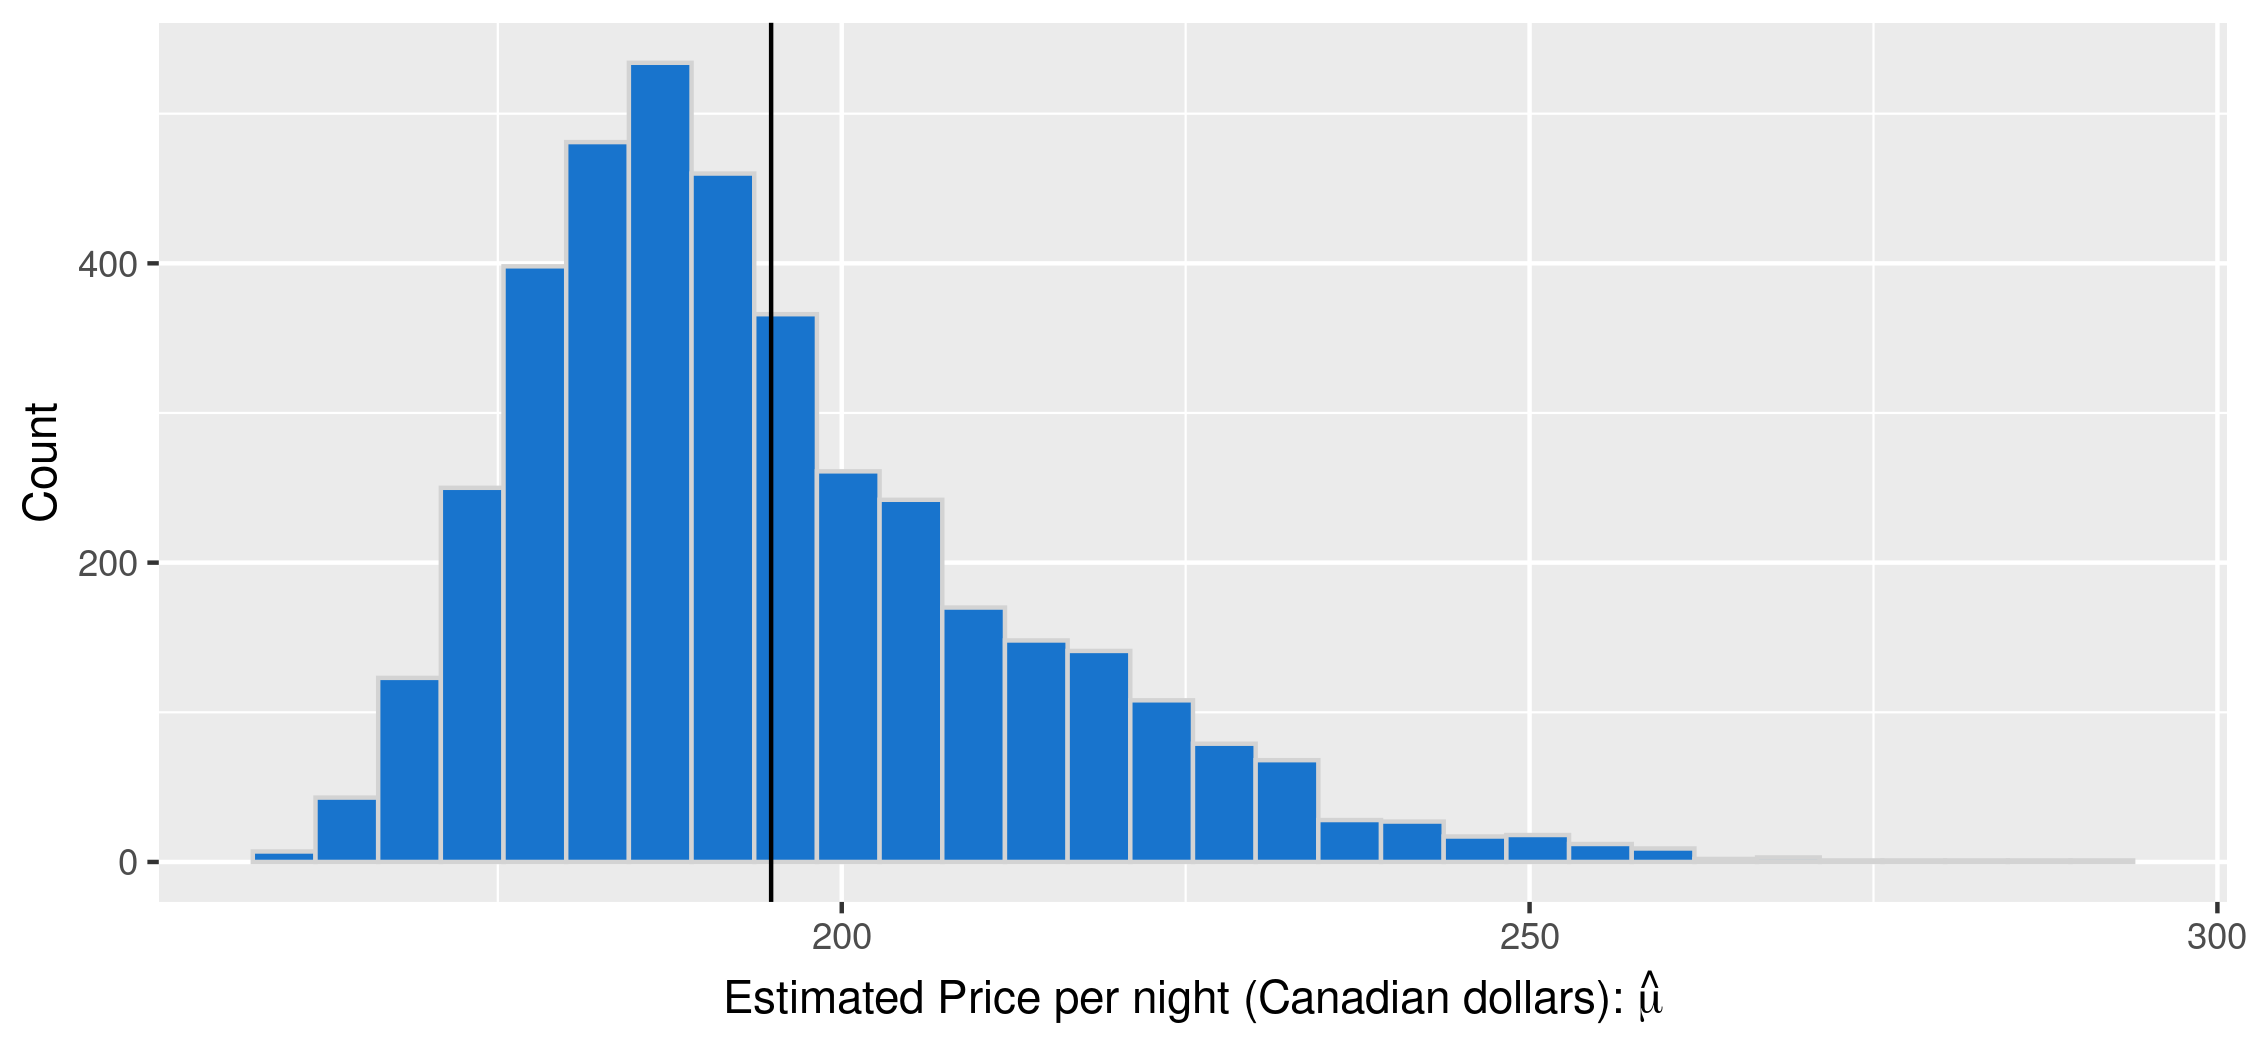
\includegraphics[width=0.98\linewidth,height=0.461\linewidth]{figure/base-hist-1} 

}



\end{knitrout}
}


\newcommand{\BaseHistogramWithArrow}{
\begin{knitrout}
\definecolor{shadecolor}{rgb}{0.969, 0.969, 0.969}\color{fgcolor}

{\centering 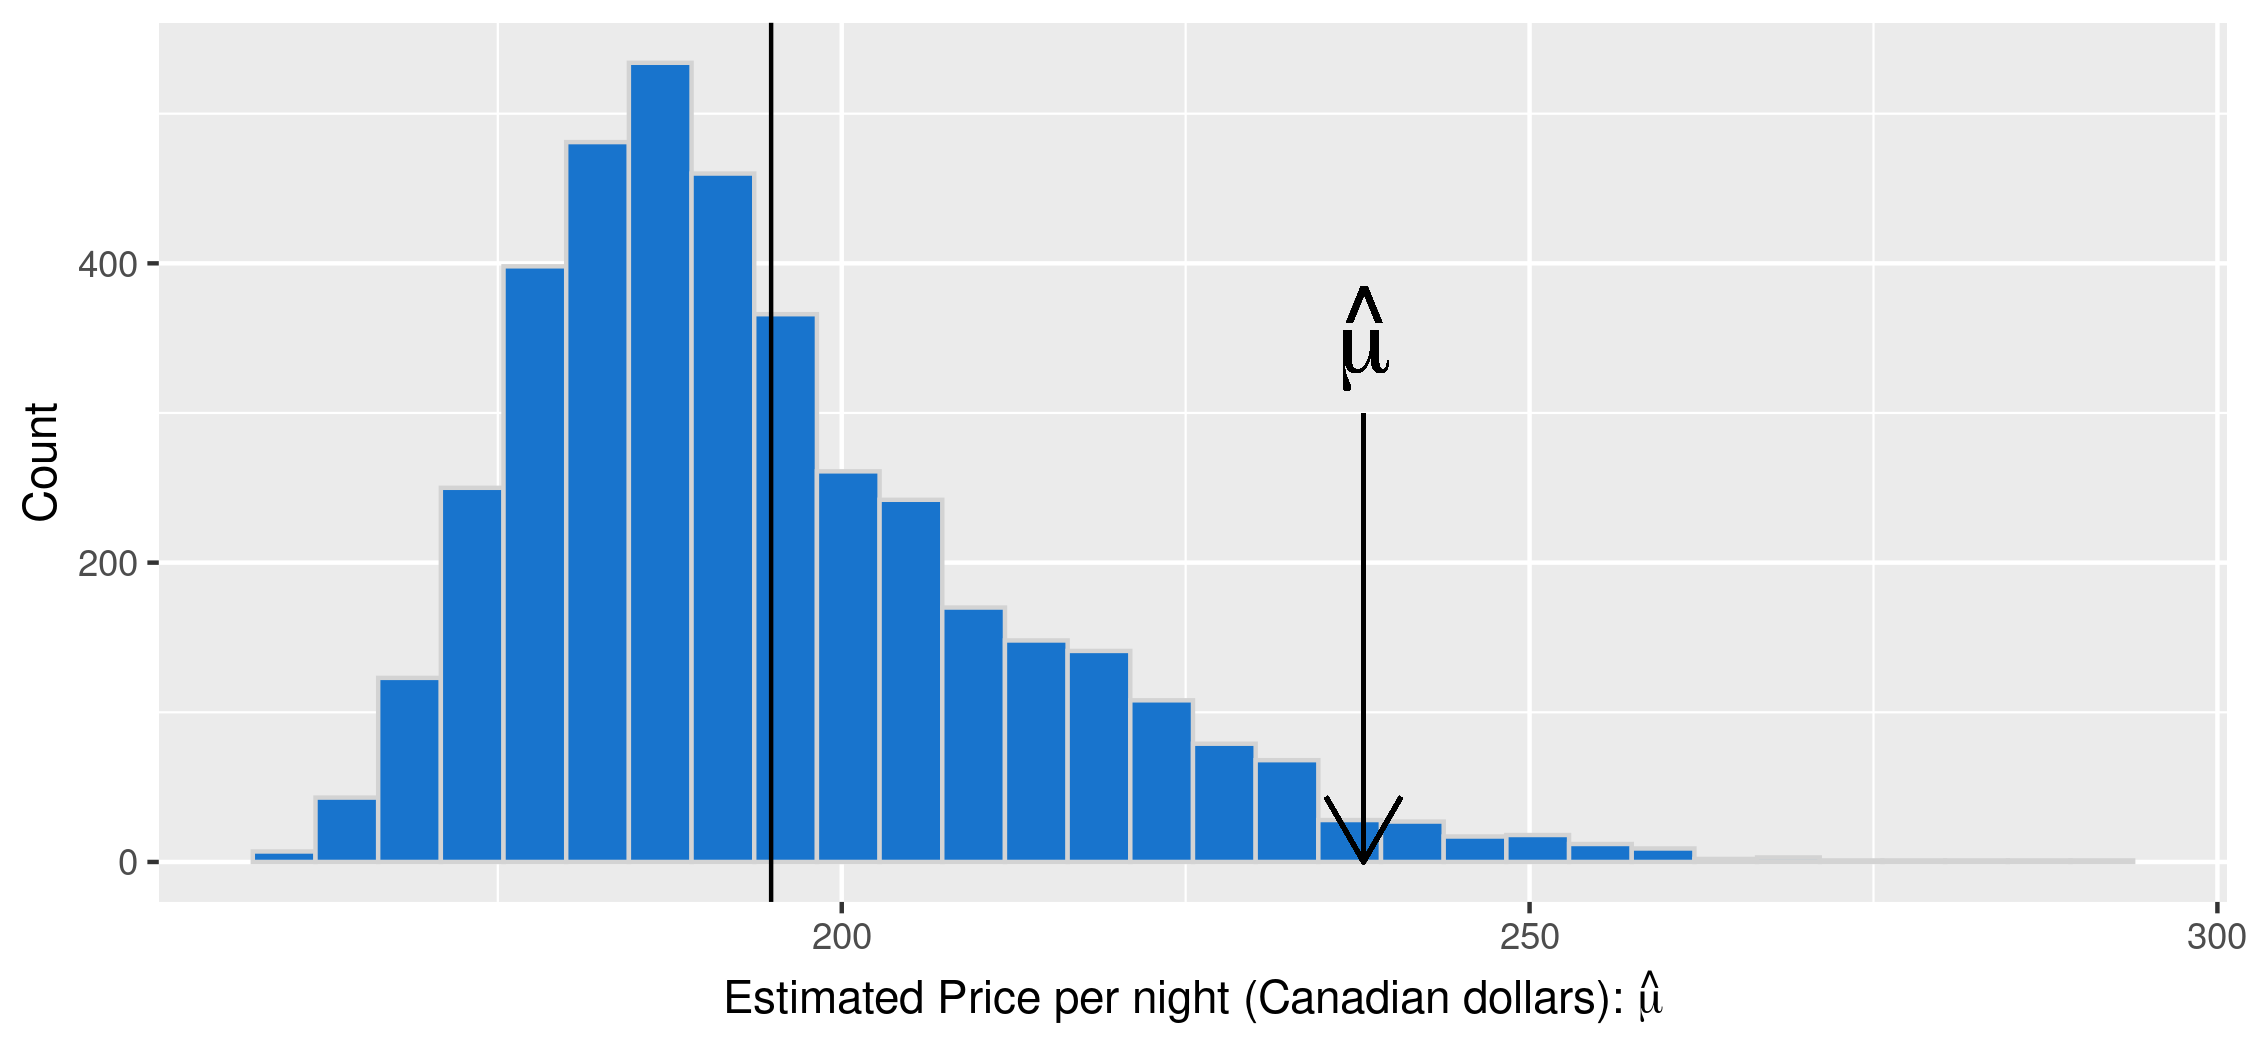
\includegraphics[width=0.98\linewidth,height=0.461\linewidth]{figure/base-hist-arrow-1} 

}



\end{knitrout}
}



\newcommand{\BaseHistogramFaded}{
\begin{knitrout}
\definecolor{shadecolor}{rgb}{0.969, 0.969, 0.969}\color{fgcolor}

{\centering 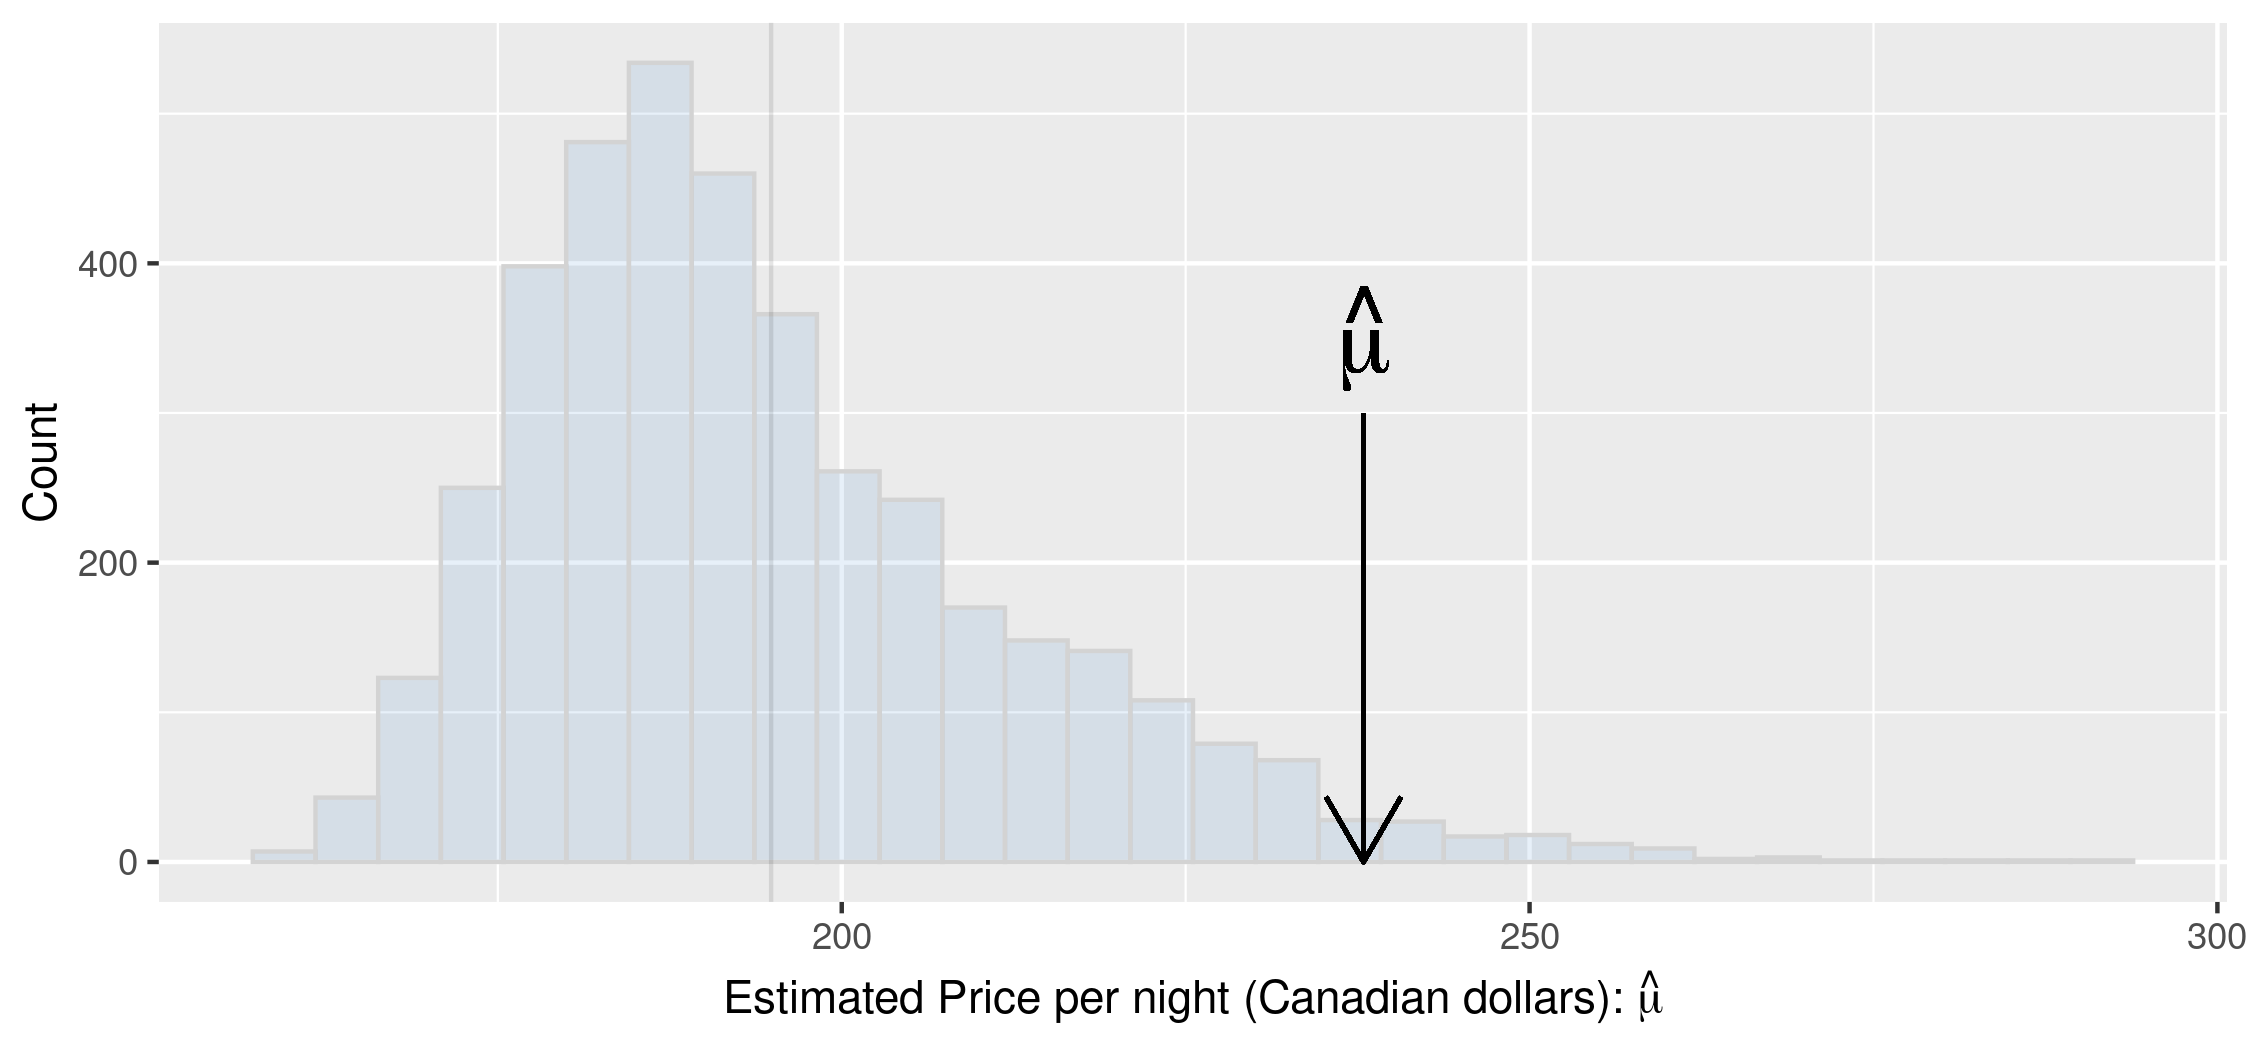
\includegraphics[width=0.98\linewidth,height=0.461\linewidth]{figure/base-hist-faded-1} 

}



\end{knitrout}
}


\newcommand{\SingleCI}{
\begin{knitrout}
\definecolor{shadecolor}{rgb}{0.969, 0.969, 0.969}\color{fgcolor}

{\centering 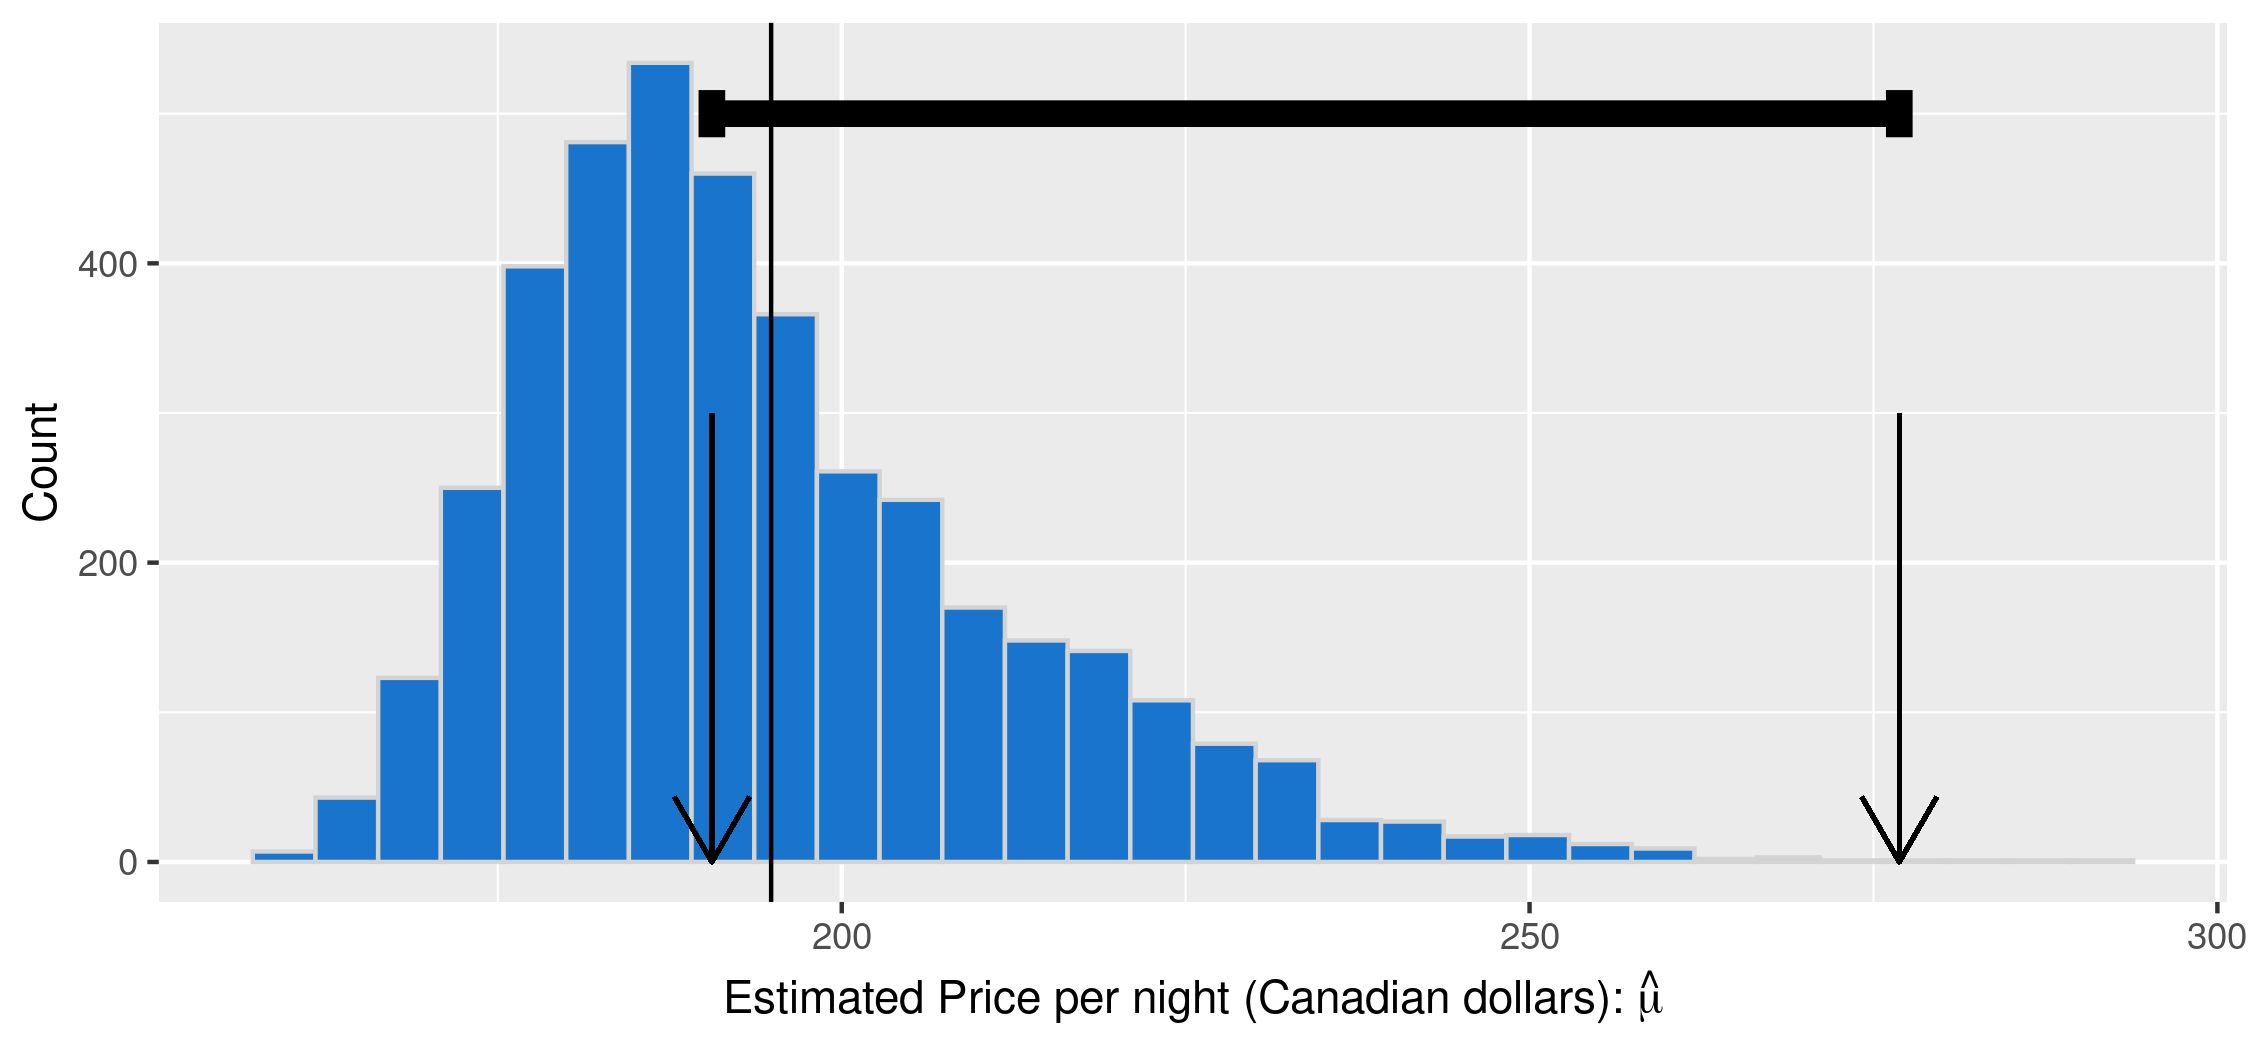
\includegraphics[width=0.98\linewidth,height=0.461\linewidth]{figure/base-hist-ci-1} 

}



\end{knitrout}
}




\newcommand{\SingleCIB}{
\begin{knitrout}
\definecolor{shadecolor}{rgb}{0.969, 0.969, 0.969}\color{fgcolor}

{\centering 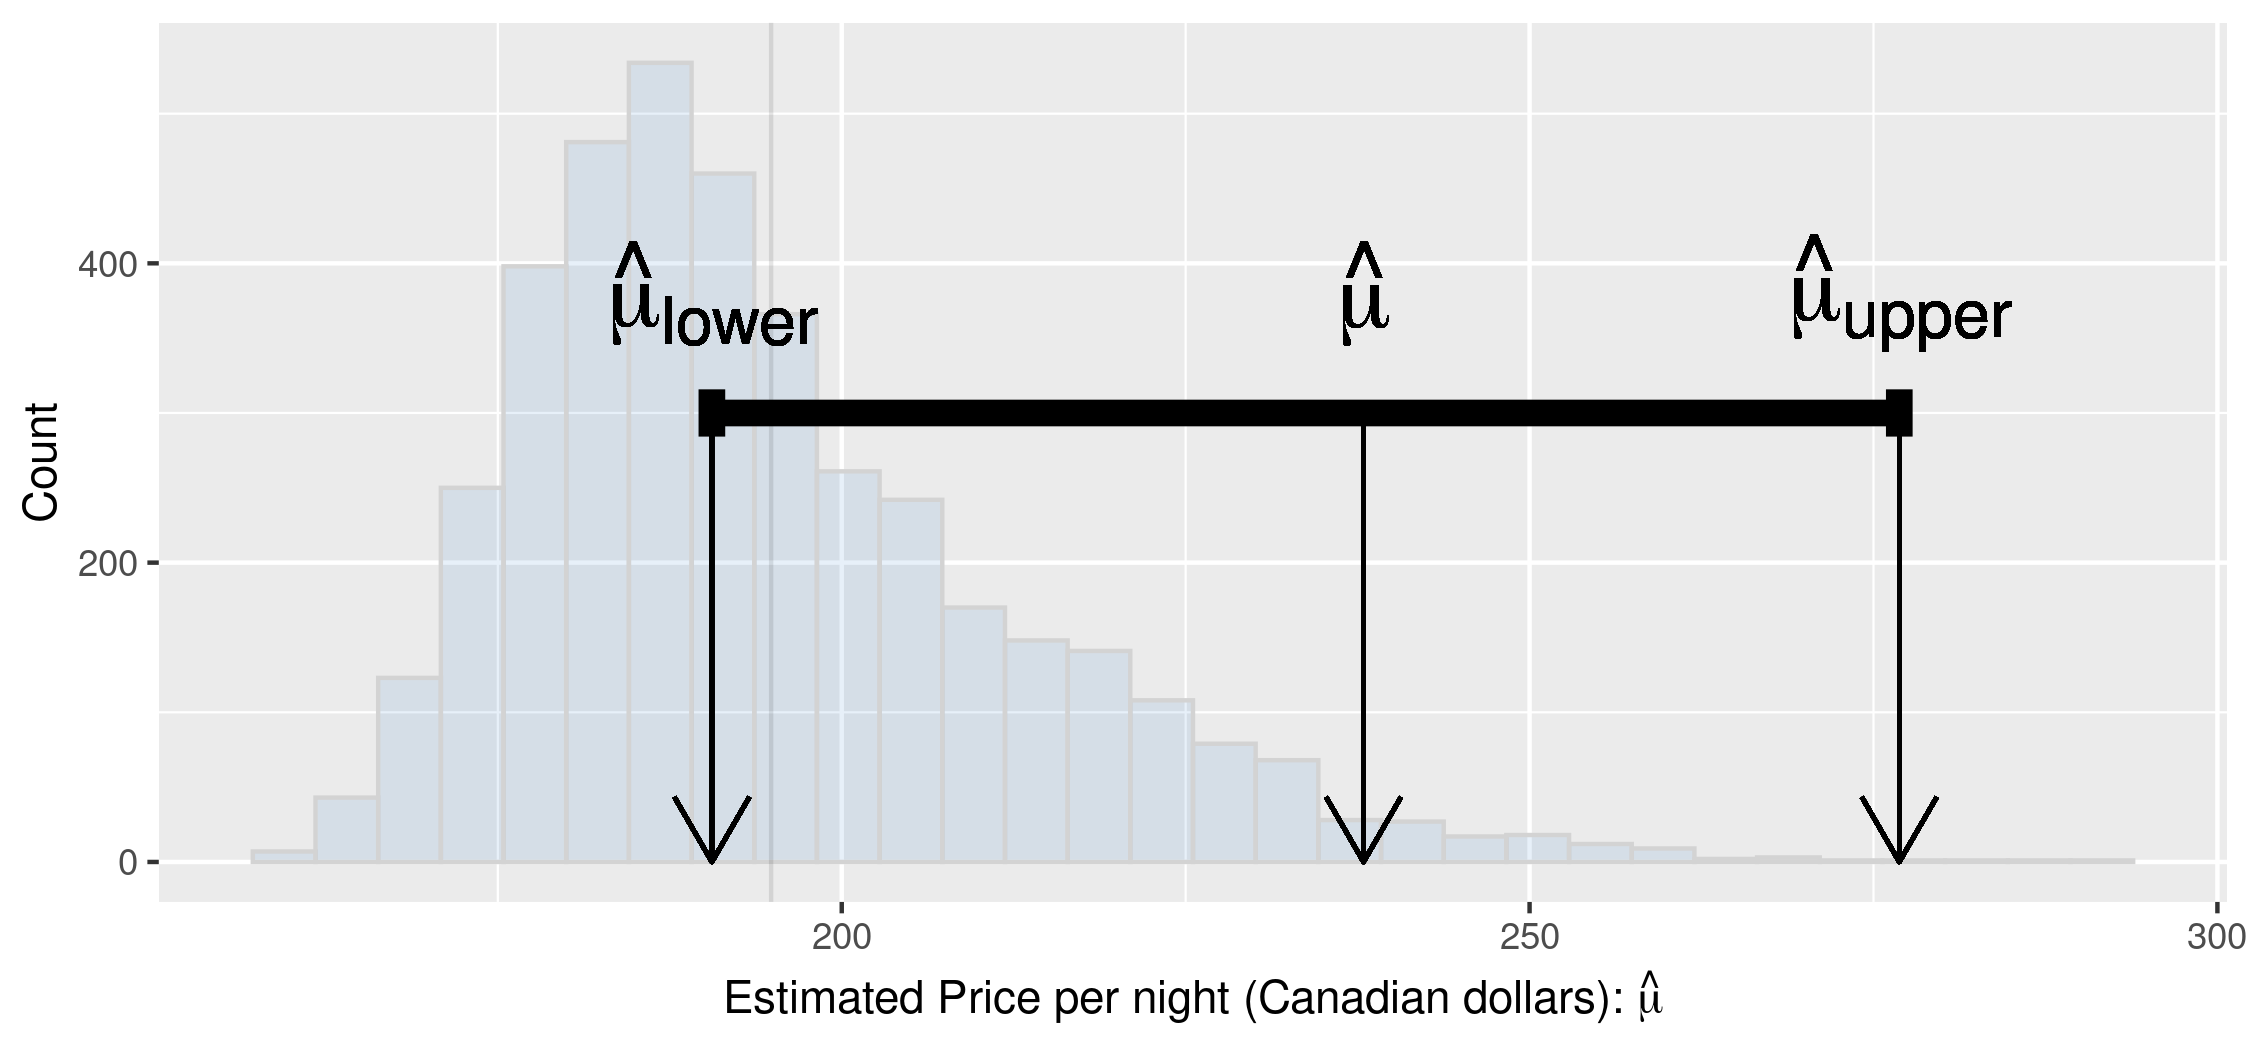
\includegraphics[width=0.98\linewidth,height=0.461\linewidth]{figure/base-hist-cib-1} 

}



\end{knitrout}
}



\newcommand{\MultipleCIs}{



\begin{knitrout}
\definecolor{shadecolor}{rgb}{0.969, 0.969, 0.969}\color{fgcolor}

{\centering 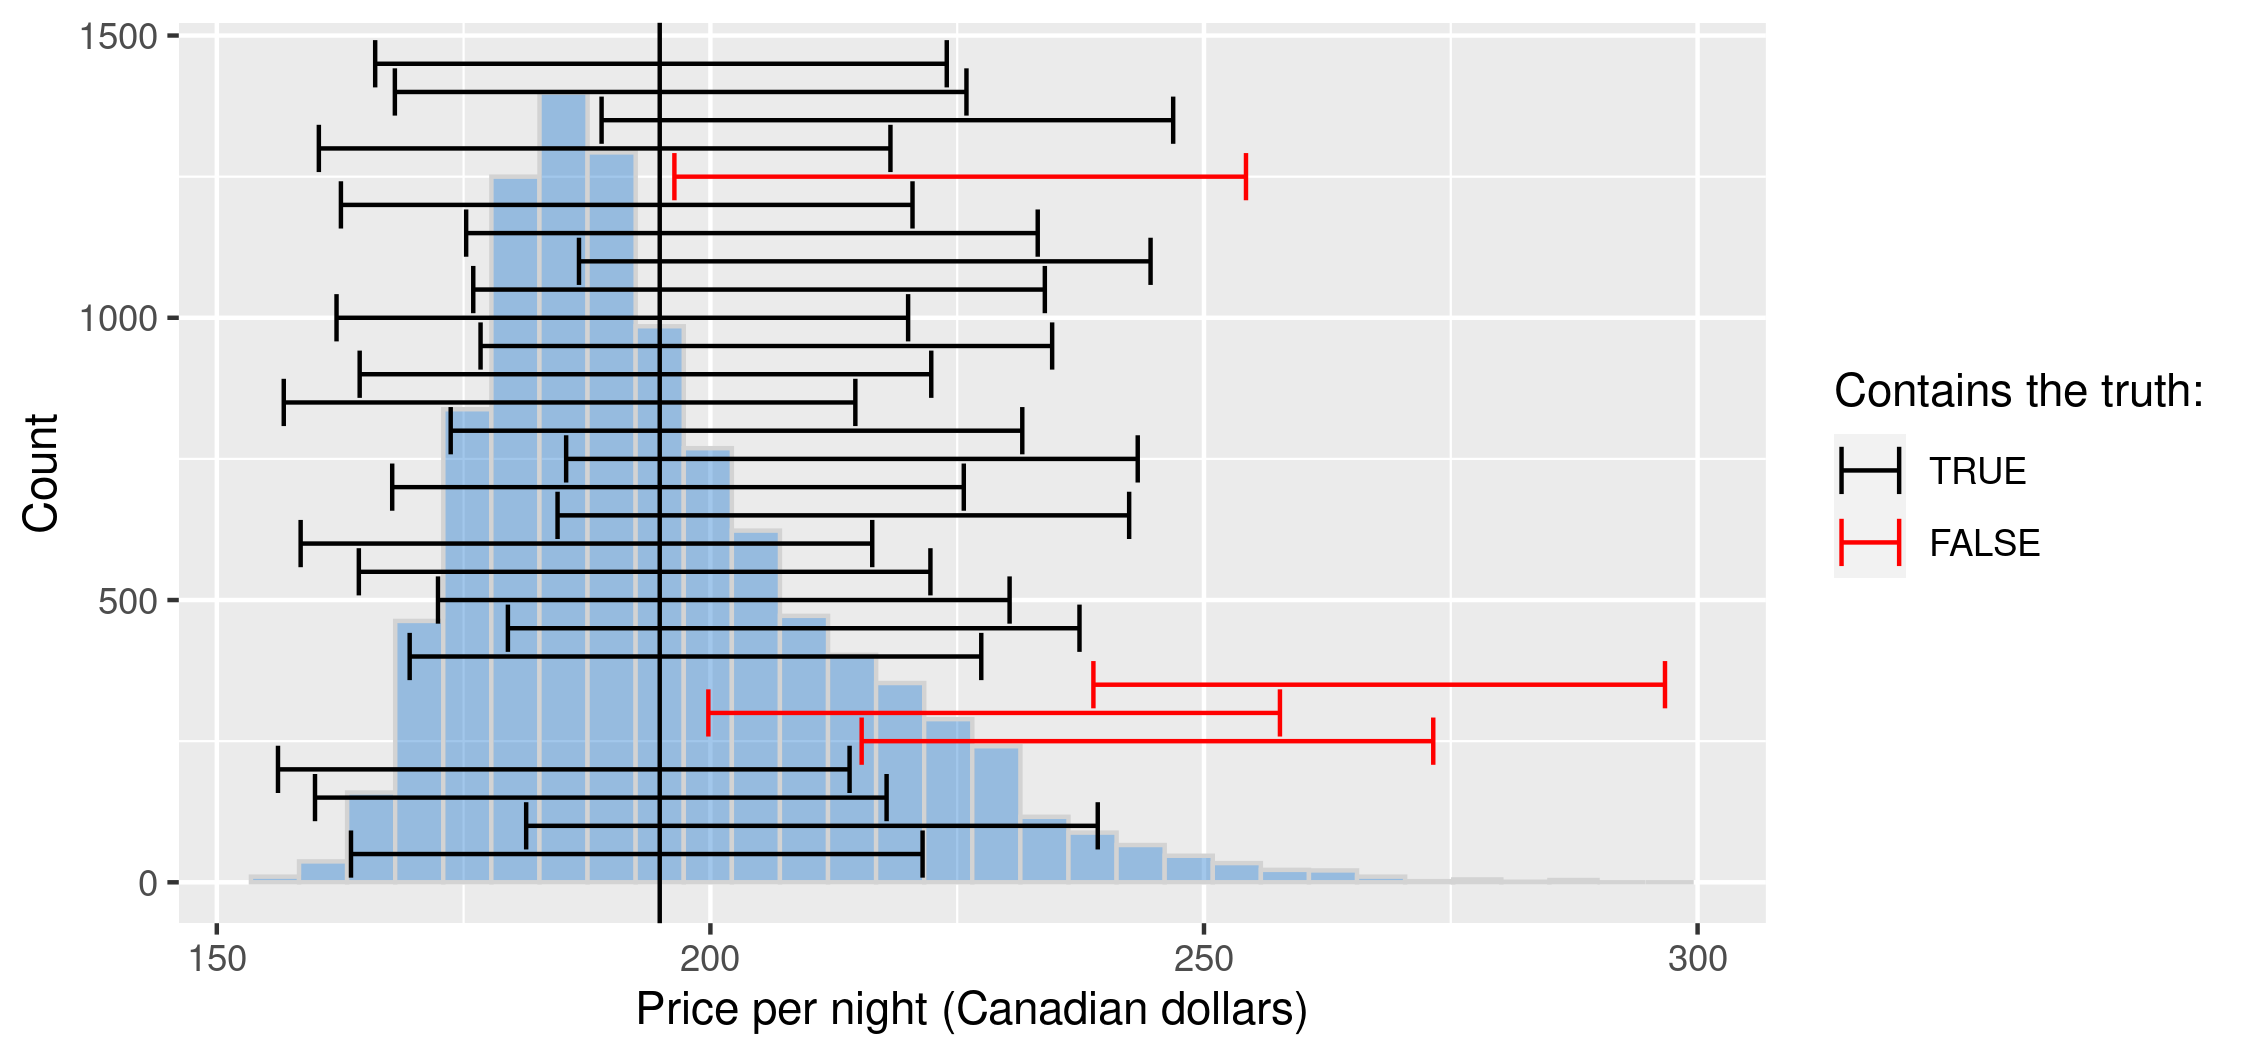
\includegraphics[width=0.98\linewidth,height=0.461\linewidth]{figure/base-hist-cis-1} 

}



\end{knitrout}
}



\begin{document}


%%%%%%%%%%%%%%%%%%%%%%%%%%%%%%%%%%%%%%%%%%%%%%%%%%%%%%%%%%%%%%%%%%%%%%%
%%%%%%%%%%%%%%%%%%%%%%%%%%%%%%%%%%%%%%%%%%%%%%%%%%%%%%%%%%%%%%%%%%%%%%%
%%%%%%%%%%%%%%%%%%%%%%%%%%%%%%%%%%%%%%%%%%%%%%%%%%%%%%%%%%%%%%%%%%%%%%%

\setbeamerfont{title}{size=\Huge}
\title{Black Box Variational Inference\\\hspace{1em}with a Deterministic Objective}

\subtitle{Faster, More Accurate, and Even More Black Box} 
\date{September 7th, 2023}

\author{Giordano, Ryan \inst{1} \and Ingram, Martin\inst{3} \and Broderick, Tamara\inst{2}}

\institute[] % (optional)
{
  \inst{1}
  University of California, Berkeley
  \and
  \inst{2}%
  Massachusetts Institute of Technology
  \and
  \inst{3}%
  University of Melbourne, Australia
}


\frame{\titlepage}

%%%%%%%%%%%%%%%%%%%%%%%%%%%%%%%%%%%%%%%%%%%%%%%%%%%%%%%%%%%%%%%%%%%%%%%
%%%%%%%%%%%%%%%%%%%%%%%%%%%%%%%%%%%%%%%%%%%%%%%%%%%%%%%%%%%%%%%%%%%%%%%
%%%%%%%%%%%%%%%%%%%%%%%%%%%%%%%%%%%%%%%%%%%%%%%%%%%%%%%%%%%%%%%%%%%%%%%

\begin{frame}{Problem statement}

We all want to do accurate Bayesian inference quickly:
%
\begin{itemize}
    \item In terms of compute (wall time, model evaluations, parallelism)
    \item In terms of analyst effort (tuning, algorithmic complexity)
\end{itemize}
%
\textbf{Markov Chain Monte Carlo (MCMC)} can be
straightforward and accurate but slow.

\pause
\vspace{-0.5em}
\hrulefill

\textbf{Black Box Variational Inference (BBVI)} can be faster alternative to MCMC.
%
\textbf{But...}

%
\begin{itemize}
    \item BBVI is cast as an optimization problem with an intractable objective $\Rightarrow$
    \item Most BBVI methods use \textbf{stochastic gradient} (SG) optimization $\Rightarrow$
    %
    \begin{itemize}
        \item SG algorithms can be hard to tune
        \item Assessing convergence and stochastic error can be difficult
        \item SG optimization can perform worse than second-order methods on tractable objectives
    \end{itemize}
    %
    \item Many BBVI methods employ a \textbf{mean-field (MF) approximation} $\Rightarrow$
    %
    \begin{itemize}
        \item Posterior variances are poorly estimated
    \end{itemize}
    %
\end{itemize}
%
\pause
\vspace{-0.5em}
\hrulefill

\textbf{Our proposal:}
replace the intractable BBVI objective with a fixed approximation.
%
\begin{itemize}
    \item Better optimization methods can be used (e.g. true second-order methods)
    \item Convergence and approximation error can be assessed directly
    \item Can correct posterior covariances with linear response covariances
    \item This technique is well-studied (but there's still work to do in the context of BBVI)
\end{itemize}
%
$\Rightarrow$
\textbf{Simpler, faster, and better BBVI posterior approximations ... in some cases.}
%
\end{frame}


%%%%%%%%%%%%%%%%%%%%%%%%%%%%%%%%%%%%%%%%%%%%%%%%%%%%%%%%%%%%%%%%%%%%%%%%%%%%%%%%%%%%%
%%%%%%%%%%%%%%%%%%%%%%%%%%%%%%%%%%%%%%%%%%%%%%%%%%%%%%%%%%%%%%%%%%%%%%%%%%%%%%%%%%%%%
%%%%%%%%%%%%%%%%%%%%%%%%%%%%%%%%%%%%%%%%%%%%%%%%%%%%%%%%%%%%%%%%%%%%%%%%%%%%%%%%%%%%%

\begin{frame}{Outline}
%
\begin{itemize}
    \item BBVI Background and our proposal
    \begin{itemize}
        \item Automatic differentiation variational inference (ADVI) (a BBVI method)
        \item Our approximation: ``Deterministic ADVI'' (DADVI)
        \item Linear response (LR) covariances
        \item Estimating approximation error
    \end{itemize}
    \item Experimental results: DADVI vs ADVI
    \begin{itemize}
        \item DADVI converges faster than ADVI, and requires no tuning
        \item DADVI's posterior mean estimates' accuracy are comparable to ADVI
        \item DADVI+LR provides more accurate posterior variance estimates than ADVI
        \item DADVI provides accurate estimates of its own approximation error
        \item But stochastic ADVI often results in better objective function values (eventually)
    \end{itemize}
    \item Theory and shortcomings
    \begin{itemize}
        \item Pessimistic dimension dependence results from optimization theory
        \item ...which do not apply in certain BBVI settings.
        \item DADVI fails for expressive BBVI approximations (e.g. full-rank ADVI)
        \item More work to be done!
    \end{itemize}
\end{itemize}
%
\end{frame}

%%%%%%%%%%%%%%%%%%%%%%%%%%%%%%%%%%%%%%%%%%%%%%%%%%%%%%%%%%%%%%%%%%%%%%%%%%%%%%%%%%%%%
%%%%%%%%%%%%%%%%%%%%%%%%%%%%%%%%%%%%%%%%%%%%%%%%%%%%%%%%%%%%%%%%%%%%%%%%%%%%%%%%%%%%%
%%%%%%%%%%%%%%%%%%%%%%%%%%%%%%%%%%%%%%%%%%%%%%%%%%%%%%%%%%%%%%%%%%%%%%%%%%%%%%%%%%%%%

\begin{frame}[t]{Notation}
%
\vspace{-2em}
%
\begin{align*}
    \text{Data:}&\quad \y \\
    \text{Likelihood:}&\quad\p(\y \vert \theta)\\
    \text{Parameter:}& \quad \theta \in \mathbb{R}^{\thetadim}\\
    \text{Prior:}&\quad \p(\theta) 
        \quad \text{(density w.r.t. Lebesgue $\mathbb{R}^\thetadim$, 
            nonzero everywhere)}\\
\end{align*}
%
We will be interested in means and covariances of the posterior $\post$.

\pause
%
% Denote gradients with $\nabla$, e.g.,
% %
% \begin{align*}
% %
% \logjointgrad := \fracat{\partial \logjoint}{\partial \theta}{\theta}
% \quad\text{and}\quad
% \logjointhess := \fracat{\partial^2 \logjoint}
%     {\partial \theta \partial \theta^\trans}{\theta}
% %
% \end{align*}

'%

\begin{minipage}{0.35\textwidth}
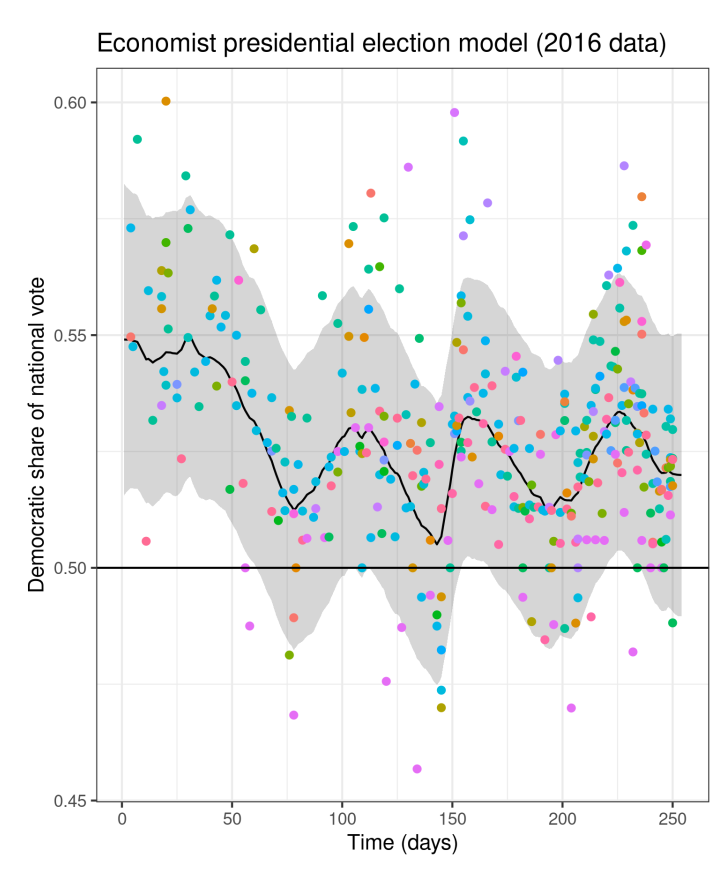
\includegraphics[width=\linewidth]{static_figures/election_data}
\end{minipage}
\begin{minipage}{0.63\textwidth}
    Example: Election modeling (2016 US POTUS)
    %
    \begin{align*}
        \text{Data } \y:&\quad \textrm{Polling data (colored dots)} \\
        \text{Likelihood } \p(\y \vert \theta):&\quad \textrm{Time series with random effects}\\
        \text{Parameter }\theta:& \quad \PotusParamDim\textrm{-dimensional}\\
        \text{Interested in:}& \quad\textrm{Vote share on election day}\\
        \text{MCMC time:}& \quad \PotusNUTSMinutes \textrm{ minutes (PyMC3 NUTS)}
    \end{align*}

    \textbf{How can we approximate the posterior more quickly?}

    \textbf{One answer: variational inference.}

\end{minipage}

\end{frame}


%%%%%%%%%%%%%%%%%%%%%%%%%%%%%%%%%%%%%%%%%%%%%%%%%%%%%%%%%%%%%%%%%%%%%%%%%%%%%%%%%%%%%
%%%%%%%%%%%%%%%%%%%%%%%%%%%%%%%%%%%%%%%%%%%%%%%%%%%%%%%%%%%%%%%%%%%%%%%%%%%%%%%%%%%%%
%%%%%%%%%%%%%%%%%%%%%%%%%%%%%%%%%%%%%%%%%%%%%%%%%%%%%%%%%%%%%%%%%%%%%%%%%%%%%%%%%%%%%

\begin{frame}[t]{Variational inference \citep{blei:2016:variational}}
%
We want the posterior $\post$.  Let $\kl{\q(\theta)}{\p(\theta)}$ denote KL divergence:
%
\begin{align*}
    \kl{\q(\theta)}{\p(\theta)} = \expect{\q(\theta)}{\log \q(\theta)} - \expect{\q(\theta)}{\log \p(\theta)}.
\end{align*}
%
The KL divergence is zero if and only if the two distributions are the same.

\pause

%
\begin{align*}
%
\textrm{A tautology: }&& \post &= \argmin_{\q} \kl{\q(\theta)}{\post} \\
\textrm{Variational inference: }&& \qstar(\theta) &= \argmin_{\q \in \qdom} \kl{\q(\theta)}{\post}
\quad\textrm{ ... for restricted }\qdom\\
%
\end{align*}
%
\pause
%
\begin{minipage}{0.4\textwidth}
    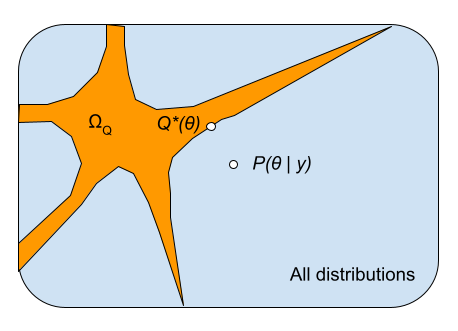
\includegraphics[width=\textwidth]{static_figures/VB}
\end{minipage}
\begin{minipage}{0.55\textwidth}
We hope to choose $\qdom$ so that
%
\begin{itemize}
\item The optimization problem is tractable
%
\begin{itemize}
\item[$\rightarrow$] simple $\qdom$ are better
\end{itemize}
%
\item The best approximation is a good one
\begin{itemize}
    \item[$\rightarrow$] complex $\qdom$ are better
\end{itemize}    
\end{itemize}

The approximation can be poor because
%
\begin{itemize}
\item Poor optimization
\item The family $\qdom$ isn't expressive enough
\end{itemize}
%
%
\end{minipage}
\end{frame}


% %%%%%%%%%%%%%%%%%%%%%%%%%%%%%%%%%%%%%%%%%%%%%%%%%%%%%%%%%%%%%%%%%%%%%%%%%%%%%%%%%%%%%
% %%%%%%%%%%%%%%%%%%%%%%%%%%%%%%%%%%%%%%%%%%%%%%%%%%%%%%%%%%%%%%%%%%%%%%%%%%%%%%%%%%%%%
% %%%%%%%%%%%%%%%%%%%%%%%%%%%%%%%%%%%%%%%%%%%%%%%%%%%%%%%%%%%%%%%%%%%%%%%%%%%%%%%%%%%%%


\begin{frame}{When does variational inference work?}

When, in general, is $\qstar(\theta)$ a good approximation for a given family $\qdom$?  

\vspace{1em}

\textbf{It is hard to say.}

\end{frame}


% %%%%%%%%%%%%%%%%%%%%%%%%%%%%%%%%%%%%%%%%%%%%%%%%%%%%%%%%%%%%%%%%%%%%%%%%%%%%%%%%%%%%%
% %%%%%%%%%%%%%%%%%%%%%%%%%%%%%%%%%%%%%%%%%%%%%%%%%%%%%%%%%%%%%%%%%%%%%%%%%%%%%%%%%%%%%
% %%%%%%%%%%%%%%%%%%%%%%%%%%%%%%%%%%%%%%%%%%%%%%%%%%%%%%%%%%%%%%%%%%%%%%%%%%%%%%%%%%%%%


\begin{frame}[t]{Black-box variational inference}

To perform VI, we need to solve
%
\begin{align*}
%
\qstar(\theta) &= \argmin_{\q \in \qdom} 
\undernote{
\left( 
\undernote{
    \expect{\q(\theta)}{\log \q(\theta)}
    }{\textrm{Entropy of }\q} - 
\undernote{
    \expect{\q(\theta)}{\log \p(\theta, \y)}
}{\textrm{Often intractable}}
 - \overnote{\p(\y)}{\textrm{Constant}}
\quad\right)}{\kl{\q(\theta)}{\p(\theta)}}.
%
\end{align*}

How can we optimize this objective?
\pause
\textbf{Black-box VI \citep{ranganath:2014:bbvi}: }
%
\begin{itemize}
    \item Parameterize the family $\qdom$ using $\eta \in \rdom{\etadim}$ (so we have $\q(\theta \vert \eta)$)
    \begin{itemize}
        \item We will study \textbf{ADVI}, which takes $\q(\theta \vert \eta)$
        to be Gaussian
        \citep{kucukelbir:2017:advi}.
        \item The parameters $\eta$ are the means and covariance (``mean-field'' or ``full-rank'')
    \end{itemize}
    \item Re-write the objective (using the reparameterization trick) as 
    \begin{align*}
        %
        \argmin_{\eta} F(\eta)
        \quad\text{ where }\quad F(\eta) := \expect{\normz}{f(\eta, \z)}.
        %
    \end{align*}
    \item Use autodiff to differentiate $\eta \mapsto f(\eta, \z)$
    \item Optimize with stochastic optimization using draws $\z_n \sim \normz$.
\end{itemize}

% \pause
% \vspace{3em}
% \textbf{In the old days \citep{bishop:2006:pattern}: }Restrict to models with tractable expectations.

% \pause
% \vspace{3em}
% These days we use 

%   Assume that 
% %
% \begin{itemize}
%     \item We can sample from $\q(\theta)$ and evaluate $\log \q(\theta)$
%     \item We have a twice auto-differentiable software implementation of $\logjoint$
% \end{itemize}
% %
% Then use stochastic optimization.


% \begin{itemize}
%     \item Use a multivariate normal family (either ``mean field'' or full-rank).
%     \item Use the ``reparameterization trick'' to write the KL using $\normz$
%     \item Do SGD using draws from $\normz$
% \end{itemize}

\pause
\hrulefill

\blue{\textbf{We propose:}}\\Instead of \red{$\expect{\normz}{f(\eta, \z)}$},
optimize \blue{$\meann f(\eta, \z_n)$} for fixed $\z_n \iid \normz$.


% ADVI specifies a family $\qdom$ of $\thetadim$-dimensional Gaussian
% distributions, parameterized by $\eta \in \etadom$, encoding the means and
% covariances.
% %
% The covariances can either be
% %
% \begin{itemize}
% \item Diagonal: ``Mean-field'' (MF) approximation, $\etadim = 2 \thetadim$
% \item Any PD matrix: 
%     ``Full-rank'' (FR) approximation, 
%         $\etadim = \thetadim + \thetadim  (\thetadim - 1) / 2$
% \end{itemize}
%

\end{frame}



    
%%%%%%%%%%%%%%%%%%%%%%%%%%%%%%%%%%%%%%%%%%%%%%%%%%%%%%%%%%%%%%%%%%%%%%%%%%%%%%%%%%%%%
%%%%%%%%%%%%%%%%%%%%%%%%%%%%%%%%%%%%%%%%%%%%%%%%%%%%%%%%%%%%%%%%%%%%%%%%%%%%%%%%%%%%%
%%%%%%%%%%%%%%%%%%%%%%%%%%%%%%%%%%%%%%%%%%%%%%%%%%%%%%%%%%%%%%%%%%%%%%%%%%%%%%%%%%%%%


% \begin{frame}[t]{Notation}
% %
% % \begin{align*}
% %     \text{Parameter: }& \theta \in \mathbb{R}^{\thetadim} &
% %     \text{Data: }& \y &
% %     \text{Log joint: }& \logjoint
% % \end{align*}
% % \hrulefill


% We will study \textbf{ADVI}, a particular BBVI method
% \citep{kucukelbir:2017:advi}.

% ADVI specifies a family $\qdom$ of $\thetadim$-dimensional Gaussian
% distributions, parameterized by $\eta \in \etadom$, encoding the means and
% covariances.
% %
% The covariances can either be
% %
% \begin{itemize}
% \item Diagonal: ``Mean-field'' (MF) approximation, $\etadim = 2 \thetadim$
% \item Any PD matrix: 
%     ``Full-rank'' (FR) approximation, 
%         $\etadim = \thetadim + \thetadim  (\thetadim - 1) / 2$
% \end{itemize}
% %

% \pause
% \hrulefill

% ADVI tries to find
% %
% \begin{align*}
% %
% \argmin_{\q \in \qdom} 
% \mathrm{KL}\left(\q(\theta | \eta) || \post \right) ={}&
% \argmin_{\eta \in \etadom} \klfullobj{\eta} 
% \quad\textrm{where }\\
% \klfullobj{\eta} :={}&
% % \expect{\q(\theta \vert \eta)}{\log \q(\theta \vert \eta)}
% % -\expect{\q(\theta \vert \eta)}{\logjoint}
% \undernote{\expect{\normz}{\log \q(\theta(\z, \eta) \vert \eta)}}
% {\text{Available in closed form}} -
% \undernote{\expect{\normz}{\log \p(\theta(\z, \eta), \y)}}
% {\red{\text{Typically intractable}}}.
% %
% \end{align*}
% %
% The final line uses the ``reparameterization trick''
% with standard Gaussian $\z \sim \normz$. 

% \pause
% \hrulefill

% ADVI is an instance of the \textit{general problem} of finding
% %
% \begin{align*}
% %
% \argmin_{\eta} F(\eta)
% \quad\text{ where }\quad F(\eta) := \expect{\normz}{f(\eta, \z)}.
% %
% \end{align*}


% \end{frame}


%%%%%%%%%%%%%%%%%%%%%%%%%%%%%%%%%%%%%%%%%%%%%%%%%%%%%%%%%%%%%%%%%%%%%%%%%%%%%%%%%%%%%
%%%%%%%%%%%%%%%%%%%%%%%%%%%%%%%%%%%%%%%%%%%%%%%%%%%%%%%%%%%%%%%%%%%%%%%%%%%%%%%%%%%%%
%%%%%%%%%%%%%%%%%%%%%%%%%%%%%%%%%%%%%%%%%%%%%%%%%%%%%%%%%%%%%%%%%%%%%%%%%%%%%%%%%%%%%


\begin{frame}{Two approaches}
%
%
\vspace{-1em}
\begin{align*}
%
\text{Consider }\quad
\argmin_{\eta} F(\eta)
\quad\text{ where } \quad F(\eta) := \expect{\normz}{f(\eta, \z)}.
%
\end{align*}
%
Let $\Z = \{\z_1, \ldots, \z_\znum \} \iid \normz$, and let
%
%\begin{align*}
%
$
\hat{F}(\eta | \Z) := \meann f(\eta, \z_n).
$
%
%\end{align*}
%
%
\begin{minipage}{1.0\linewidth}
    \begin{minipage}[t]{0.49\linewidth}
        %
        \onslide<2->{
        \begin{algorithm}[H]
        \caption{\\Stochastic gradient (SG)\\ADVI (and most BBVI)}
        \begin{algorithmic}
        % \Procedure{SG}{}
        \State Fix $\znum$ (typically $\znum = 1$)
        \State $t \gets 0$
            \While{Not converged}
                \State $t \gets t + 1$
                \red{\State Draw $\Z$}
                \blue{
                    \State $\Delta_S \gets \grad{\eta}{\hat{F}(\eta_{t-1} | \Z)}$
                    \State $\alpha_t \gets \textrm{SetStepSize(Past state)}$
                    \State $\eta_t \gets \eta_{t-1} - \alpha_t \Delta_S$
                }
                \green{\State $\textrm{AssessConvergence(Past state)}$}
            \EndWhile
            % \State $\etaopts \gets \eta_t$ or
            %     $\etaopts \gets \frac{1}{M} \sum_{t'=t- M}^t \eta_{t'}$
            \State \Return 
            $\eta_t$ or
                $\frac{1}{M} \sum_{t'=t- M}^t \eta_{t'}$
        % \EndProcedure
        \end{algorithmic}
        \end{algorithm}
        } % Onslide
        %
    \end{minipage}
    \begin{minipage}[t]{0.49\linewidth}
        %
        \onslide<3->{
        \begin{algorithm}[H]
        \caption{\\Sample average approximation (SAA)\\Deterministic ADVI (DADVI) (proposal)}\label{alg:dadvi}
        \begin{algorithmic}
        % \Procedure{DADVI}{}
            \State Fix $\znum$ (our experiments use $\znum = 30$)
            \State \red{Draw $\Z$}
            \State $t \gets 0$
            \While{Not converged}
                \State $t \gets t + 1$
                \blue{
                    \State
                    $\Delta_D \gets \textrm{GetStep}(\hat{F}(\cdot | \Z), \eta_{t-1})$
                    \State $\eta_t \gets \eta_{t-1} + \Delta_D$
                    }
                \State \green{$\textrm{AssessConvergence}(\hat{F}(\cdot | \Z), \eta_{t})$}
            \EndWhile
            % \State $\etaoptd \gets \eta_t$
            \State \Return $\eta_t$
        \end{algorithmic}
        \end{algorithm}
        } % Onslide
    \end{minipage}
\end{minipage}

% \begin{minipage}{1.0\linewidth}
%     \begin{minipage}[t]{0.49\linewidth}
%         {\small ADVI approximately minimizes an exact objective.}
%     \end{minipage}    
%     \begin{minipage}[t]{0.49\linewidth}
%         SAA exactly minimizes an approximate objective.
%     \end{minipage}    
% \end{minipage}    

\onslide<4->{
\textbf{Our proposal: } Apply Algorithm 2 with the ADVI objective.  \\
Take \blue{better steps}, easily \green{assess convergence}, with less tuning.
}

\end{frame}


%%%%%%%%%%%%%%%%%%%%%%%%%%%%%%%%%%%%%%%%%%%%%%%%%%%%%%%%%%%%%%%%%%%%%%%%%%%%%%%%%%%%%
%%%%%%%%%%%%%%%%%%%%%%%%%%%%%%%%%%%%%%%%%%%%%%%%%%%%%%%%%%%%%%%%%%%%%%%%%%%%%%%%%%%%%
%%%%%%%%%%%%%%%%%%%%%%%%%%%%%%%%%%%%%%%%%%%%%%%%%%%%%%%%%%%%%%%%%%%%%%%%%%%%%%%%%%%%%


\begin{frame}{Experiments}

For each of a range of models (next slide), we compared:

\begin{itemize}
    %
    \item \textbf{NUTS:} The ``no-U-turn'' MCMC sampler as implemented by PyMC
    \citep{salvatier:2016:pymc3}.  We used this as the ``ground truth''
    posterior.
    \item[]
    %
    \pause
    \item \textbf{DADVI:}  We used $\znum=\DADVINumDraws$ draws for DADVI for
    each model. We optimized using an off-the-shelf second-order Newton trust region
    method (\texttt{trust-ncg} in \texttt{scipy.optimize.minimize}) with no
    tuning or preconditioning.
    %
    \pause
    \item[]
    \item[]\textbf{Stochastic ADVI methods:}
    \item Mean field ADVI: We used the PyMC implementation of
    ADVI, together with its default termination criterion (based on parameter
    differences). 
    %
    \item Full-rank ADVI: We used the PyMC implementation of
    full-rank ADVI, together with the default termination criterion for ADVI
    described above.
    %
    \item RAABBVI: To run RAABBVI, we used the public package
    \texttt{viabel}, provided
    by \citet{welandawe:2022:robustbbvi}.
    %
    \end{itemize}

We terminated unconverged stochastic ADVI after 100,000 iterations.
    

\end{frame}


%%%%%%%%%%%%%%%%%%%%%%%%%%%%%%%%%%%%%%%%%%%%%%%%%%%%%%%%%%%%%%%%%%%%%%%%%%%%%%%%%%%%%
%%%%%%%%%%%%%%%%%%%%%%%%%%%%%%%%%%%%%%%%%%%%%%%%%%%%%%%%%%%%%%%%%%%%%%%%%%%%%%%%%%%%%
%%%%%%%%%%%%%%%%%%%%%%%%%%%%%%%%%%%%%%%%%%%%%%%%%%%%%%%%%%%%%%%%%%%%%%%%%%%%%%%%%%%%%


\begin{frame}{Experiments}

    We evaluated each method on a range of models.
    
    \begin{table}[h!]
        \begin{tabular}{|x{0.15\textwidth}|x{0.13\textwidth}|x{0.25\textwidth}|x{0.3\textwidth}|}
        \hline\hline
        Model Name  & Dim $\thetadim$     & NUTS runtime & Description \\
        \hline\hline
        ARM  \newline ($\ARMNumModels$ models) &
        Median $\ARMMedParamDim$ 
            \newline(max $\ARMMaxParamDim$)&
        median $\ARMMedNUTSSeconds$ seconds \
            \newline(max $\ARMMaxNUTSMinutes$ minutes) 
            &
           A range of linear models, GLMs, and GLMMs \\
        \hline
        Microcredit & $\MCParamDim$ & $\MCNUTSMinutes$ minutes &
           Hierarchical model with heavy tails and zero inflation \\
        \hline
        Occupancy & $\OccParamDim$ & $\OccNUTSMinutes$ minutes &
           Binary regression with highly crossed random effects \\
        \hline
        Tennis & $\TennisParamDim$ & $\TennisNUTSMinutes$ minutes &
           Binary regression with highly crossed random effects \\
        \hline
        POTUS & $\PotusParamDim$ & $\PotusNUTSMinutes$ minutes &
            Autoregressive time series with random effects \\
        \hline\hline
        \end{tabular}
        \caption{Model summaries.}
        \label{tab:model_desc}
    \end{table}
        
\end{frame}

%%%%%%%%%%%%%%%%%%%%%%%%%%%%%%%%%%%%%%%%%%%%%%%%%%%%%%%%%%%%%%%%%%%%%%%%%%%%%%%%%%%%%
%%%%%%%%%%%%%%%%%%%%%%%%%%%%%%%%%%%%%%%%%%%%%%%%%%%%%%%%%%%%%%%%%%%%%%%%%%%%%%%%%%%%%
%%%%%%%%%%%%%%%%%%%%%%%%%%%%%%%%%%%%%%%%%%%%%%%%%%%%%%%%%%%%%%%%%%%%%%%%%%%%%%%%%%%%%

\begin{frame}{Comparisons}

To form a common scale for the accuracy of the
posteriors, we report:
%
\begin{align*}
\muerr_{\method} :={}& \frac{\mu_{\method} - \mu_{\nuts}}{\sigma_{\nuts}}
&
\sderr_{\method} :={}& \frac{\sigma_{\method} - \sigma_{\nuts}}{\sigma_{\nuts}}.
%
\end{align*}
%
where
%
\begin{align*}
%
\mu_{\method} :={}& \method \text{ posterior mean}
&
\sigma_{\method} :={}& \method\text{ posterior SD}.
%
\end{align*}
   
\pause
\hrulefill

We measure computational cost using both
%
\begin{itemize}
\item \textbf{Wall time} and 
\item \textbf{Number of model evaluations} (gradients, Hessian-vector products).
\end{itemize}
%

We compare achieved objective values using a large number of independent samples.

We report objective values and computation cost relative to DADVI.


\end{frame}



%%%%%%%%%%%%%%%%%%%%%%%%%%%%%%%%%%%%%%%%%%%%%%%%%%%%%%%%%%%%%%%%%%%%%%%%%%%%%%%%%%%%%
%%%%%%%%%%%%%%%%%%%%%%%%%%%%%%%%%%%%%%%%%%%%%%%%%%%%%%%%%%%%%%%%%%%%%%%%%%%%%%%%%%%%%
%%%%%%%%%%%%%%%%%%%%%%%%%%%%%%%%%%%%%%%%%%%%%%%%%%%%%%%%%%%%%%%%%%%%%%%%%%%%%%%%%%%%%

\begin{frame}{Posterior mean accuracy}
    \PosteriorMeanAccuracy{}
\end{frame}

%%%%%%%%%%%%%%%%%%%%%%%%%%%%%%%%%%%%%%%%%%%%%%%%%%%%%%%%%%%%%%%%%%%%%%%%%%%%%%%%%%%%%
%%%%%%%%%%%%%%%%%%%%%%%%%%%%%%%%%%%%%%%%%%%%%%%%%%%%%%%%%%%%%%%%%%%%%%%%%%%%%%%%%%%%%
%%%%%%%%%%%%%%%%%%%%%%%%%%%%%%%%%%%%%%%%%%%%%%%%%%%%%%%%%%%%%%%%%%%%%%%%%%%%%%%%%%%%%

\begin{frame}{Computational cost for ARM models}
\RuntimeARM{}
\end{frame}

%%%%%%%%%%%%%%%%%%%%%%%%%%%%%%%%%%%%%%%%%%%%%%%%%%%%%%%%%%%%%%%%%%%%%%%%%%%%%%%%%%%%%
%%%%%%%%%%%%%%%%%%%%%%%%%%%%%%%%%%%%%%%%%%%%%%%%%%%%%%%%%%%%%%%%%%%%%%%%%%%%%%%%%%%%%
%%%%%%%%%%%%%%%%%%%%%%%%%%%%%%%%%%%%%%%%%%%%%%%%%%%%%%%%%%%%%%%%%%%%%%%%%%%%%%%%%%%%%

\begin{frame}{Computational cost for non-ARM models}
    \RuntimeNonARM{}
\end{frame}

%%%%%%%%%%%%%%%%%%%%%%%%%%%%%%%%%%%%%%%%%%%%%%%%%%%%%%%%%%%%%%%%%%%%%%%%%%%%%%%%%%%%%
%%%%%%%%%%%%%%%%%%%%%%%%%%%%%%%%%%%%%%%%%%%%%%%%%%%%%%%%%%%%%%%%%%%%%%%%%%%%%%%%%%%%%
%%%%%%%%%%%%%%%%%%%%%%%%%%%%%%%%%%%%%%%%%%%%%%%%%%%%%%%%%%%%%%%%%%%%%%%%%%%%%%%%%%%%%

\begin{frame}{Optimization traces for ARM models}
    \TracesARM{}
\end{frame}

%%%%%%%%%%%%%%%%%%%%%%%%%%%%%%%%%%%%%%%%%%%%%%%%%%%%%%%%%%%%%%%%%%%%%%%%%%%%%%%%%%%%%
%%%%%%%%%%%%%%%%%%%%%%%%%%%%%%%%%%%%%%%%%%%%%%%%%%%%%%%%%%%%%%%%%%%%%%%%%%%%%%%%%%%%%
%%%%%%%%%%%%%%%%%%%%%%%%%%%%%%%%%%%%%%%%%%%%%%%%%%%%%%%%%%%%%%%%%%%%%%%%%%%%%%%%%%%%%

\begin{frame}{Optimization traces for non-ARM models}
    \TracesNonARM{}
\end{frame}


%%%%%%%%%%%%%%%%%%%%%%%%%%%%%%%%%%%%%%%%%%%%%%%%%%%%%%%%%%%%%%%%%%%%%%%%%%%%%%%%%%%%%
%%%%%%%%%%%%%%%%%%%%%%%%%%%%%%%%%%%%%%%%%%%%%%%%%%%%%%%%%%%%%%%%%%%%%%%%%%%%%%%%%%%%%
%%%%%%%%%%%%%%%%%%%%%%%%%%%%%%%%%%%%%%%%%%%%%%%%%%%%%%%%%%%%%%%%%%%%%%%%%%%%%%%%%%%%%

\begin{frame}{Experiment summary}

$\Rightarrow$ DADVI is faster, simpler, and the posterior means are not worse.

\vspace{3em}
\textbf{But DADVI can additionally provide:}
%
\begin{itemize}
\item Simple estimates of approximation error
\item Improved (LR) posterior covariance esimates
\end{itemize}
%

\end{frame}

%%%%%%%%%%%%%%%%%%%%%%%%%%%%%%%%%%%%%%%%%%%%%%%%%%%%%%%%%%%%%%%%%%%%%%%%%%%%%%%%%%%%%
%%%%%%%%%%%%%%%%%%%%%%%%%%%%%%%%%%%%%%%%%%%%%%%%%%%%%%%%%%%%%%%%%%%%%%%%%%%%%%%%%%%%%
%%%%%%%%%%%%%%%%%%%%%%%%%%%%%%%%%%%%%%%%%%%%%%%%%%%%%%%%%%%%%%%%%%%%%%%%%%%%%%%%%%%%%


\begin{frame}{Linear response covariances and sampling uncertainty}
%
% DADVI is faster, simpler, and the posterior means are not worse.

% \textbf{But we can do even better!}

% \hrulefill

% \textbf{Approximation Error}
\vspace{-2em}

\begin{minipage}[t]{0.48\textwidth}
    \begin{align*}
        &\text{Intractable objective:} 
        \\ \etastar %:={}& \argmin_{\eta \in \etadom} F(\eta)
            ={}& 
            \argmin_{\eta \in \etadom} \expect{\normz}{f(\eta, \z)}
    \end{align*}    
\end{minipage}
\begin{minipage}[t]{0.48\textwidth}
    \begin{align*}
        &\text{DADVI approximation:} 
        \\ \etahat(\Z) %:={}& \argmin_{\eta \in \etadom} \hat{F}(\eta | \Z)
         ={}&  \argmin_{\eta \in \etadom} \meann f(\eta, \z_n).
    \end{align*}
\end{minipage}
%

% %
% The DADVI estimator $\etahat(\Z)$ is random --- it depends
% on $\Z = (\z_1, \ldots, \z_\znum)$.

\hrulefill

What is the error of the DADVI approximation $\etahat - \etastar$?

\pause

$\Leftrightarrow$ What is the distribution of the
DADVI error $\etahat - \etastar$ under sampling of $\Z$?

\textbf{Answer: } The same as a that of any M-estimator: 
    asymptotically normal (as $\znum$ grows) 
% with covariance given in terms of 
% $\hess{\eta}{\klfullobj{\etastar}} \approx \hess{\eta}{\klobj{\etahat}}$

\pause

\hrulefill

% \textbf{Linear response covariances}

Posterior variances are often badly estimated by mean-field (MF) approximations.

Linear response (LR) covariances improve covariance estimates by computing
\textit{sensitivity} of the variational means to 
particular perturbations.  \citep{giordano:2018:covariances}

\textbf{Example: } With a correlated Gaussian $\post$,
the ADVI means are exactly correct, the ADVI variances are underestimated,
and LR covariances are exactly correct.

\pause

\hrulefill

Both DADVI error and LR covariances can be computed from the DADVI objective.

Stochastic ADVI does not produce an actual optimum of any tractable
objective, so LR and M-estimator computations are unavailable.

\end{frame}


%%%%%%%%%%%%%%%%%%%%%%%%%%%%%%%%%%%%%%%%%%%%%%%%%%%%%%%%%%%%%%%%%%%%%%%%%%%%%%%%%%%%%
%%%%%%%%%%%%%%%%%%%%%%%%%%%%%%%%%%%%%%%%%%%%%%%%%%%%%%%%%%%%%%%%%%%%%%%%%%%%%%%%%%%%%
%%%%%%%%%%%%%%%%%%%%%%%%%%%%%%%%%%%%%%%%%%%%%%%%%%%%%%%%%%%%%%%%%%%%%%%%%%%%%%%%%%%%%

\begin{frame}{Posterior standard deviation accuracy}
    \PosteriorSdAccuracy{}
\end{frame}

%%%%%%%%%%%%%%%%%%%%%%%%%%%%%%%%%%%%%%%%%%%%%%%%%%%%%%%%%%%%%%%%%%%%%%%%%%%%%%%%%%%%%
%%%%%%%%%%%%%%%%%%%%%%%%%%%%%%%%%%%%%%%%%%%%%%%%%%%%%%%%%%%%%%%%%%%%%%%%%%%%%%%%%%%%%
%%%%%%%%%%%%%%%%%%%%%%%%%%%%%%%%%%%%%%%%%%%%%%%%%%%%%%%%%%%%%%%%%%%%%%%%%%%%%%%%%%%%%

\begin{frame}{DADVI approximation error accuracy}
    \CoverageHistogram{}
\end{frame}


%%%%%%%%%%%%%%%%%%%%%%%%%%%%%%%%%%%%%%%%%%%%%%%%%%%%%%%%%%%%%%%%%%%%%%%%%%%%%%%%%%%%%
%%%%%%%%%%%%%%%%%%%%%%%%%%%%%%%%%%%%%%%%%%%%%%%%%%%%%%%%%%%%%%%%%%%%%%%%%%%%%%%%%%%%%
%%%%%%%%%%%%%%%%%%%%%%%%%%%%%%%%%%%%%%%%%%%%%%%%%%%%%%%%%%%%%%%%%%%%%%%%%%%%%%%%%%%%%

\begin{frame}[t]{Previous theoretical results}
\vspace{-3em}
\begin{minipage}[t]{0.48\textwidth}
    \begin{align*}
        &\text{Intractable objective:} 
        \\ \etastar %:={}& \argmin_{\eta \in \etadom} F(\eta)
            ={}& 
            \argmin_{\eta \in \etadom} \expect{\normz}{f(\eta, \z)}
    \end{align*}    
\end{minipage}
\begin{minipage}[t]{0.48\textwidth}
    \begin{align*}
        &\text{SAA approximation (DADVI):} 
        \\ \etahat(\Z) %:={}& \argmin_{\eta \in \etadom} \hat{F}(\eta | \Z)
            ={}&  \argmin_{\eta \in \etadom} \meann f(\eta, \z_n).
    \end{align*}
\end{minipage}

\hrulefill

The idea of optimizing $\hat{F}$ instead of SG on $F$ is old and
well-studied in the optimization literature, where $\hat{F}$
is known as the \textbf{Sample average approximation (SAA)}.

Yet SAA is rarely used for BBVI.\footnote{Some exceptions I'm aware of:
\citet{giordano:2018:covariances,giordano:2022:bnp,wycoff:2022:sparsebayesianlasso,burroni:2023:saabbvi}.}
One possible reason is the following:

% \hrulefill

\noindent
\textbf{Theorem \citep{nemirovski:2009:sgdvsfixed}:}
In general, the error of both SG and SAA scale as
$\sqrt{\thetadim / \znum}$,
where, for SG, $\znum$ is the \textit{total number of samples used}.

\pause
%
\begin{itemize}
\item For SG, each $\z_n$ gets used once (for a single gradient step)
\item For SAA, each $\z_n$ gets used once per optimization step
(of which the are many).
\item Often, in higher dimensions, SAA requires more optimization steps.
\end{itemize}
%


\noindent
\textbf{Corollary: \citep{kim:2015:guidetosaa}}
In general, for a given accuracy, the computation required for SAA 
scales worse than SG as the dimension $\thetadim$ grows.

\pause
\textbf{
But we got good results with $\thetadim$ as
high as $\PotusParamDim$ using only
only $\znum = \DADVINumDraws$.  Why?}


\end{frame}



%%%%%%%%%%%%%%%%%%%%%%%%%%%%%%%%%%%%%%%%%%%%%%%%%%%%%%%%%%%%%%%%%%%%%%%%%%%%%%%%%%%%%
%%%%%%%%%%%%%%%%%%%%%%%%%%%%%%%%%%%%%%%%%%%%%%%%%%%%%%%%%%%%%%%%%%%%%%%%%%%%%%%%%%%%%
%%%%%%%%%%%%%%%%%%%%%%%%%%%%%%%%%%%%%%%%%%%%%%%%%%%%%%%%%%%%%%%%%%%%%%%%%%%%%%%%%%%%%

\begin{frame}{Some first steps}

\noindent
\textbf{Theorem \citep{giordano:2023:dadvi}:} When $\post$ is multivariate
normal, and we use the mean-field Gaussian approximation, then, for any
particular entry $\eta_d$ of $\eta$, then $\abs{\etahat_d - \etastar_d} =
O_p(N^{-1/2})$ irrespective of $\thetadim$.

\pause
\vspace{2em}
\noindent
\textbf{Theorem \citep{giordano:2023:dadvi}:} Assume $\post$ has a ``global-local''
structure:
%
\begin{align*}
\theta ={}& (\gamma, \lambda_1, \ldots, \lambda_\lambdadim) &
\p(\gamma, \lambda_1, \ldots, \lambda_\lambdadim | \y) ={}&
\prod_{d=1}^{\lambdadim} \p(\gamma, \lambda_d \vert \y).
\end{align*}
%
Assume that the dimension of $\gamma$ and each $\lambda_d$ stays fixed as
$\lambdadim$ grows.

Under regularity conditions, the DADVI error
scales as $\sqrt{\log \lambdadim / \znum}$, not $\sqrt{\lambdadim / \znum}$.

\vspace{2em}

\pause
\noindent
\textbf{Proposal: }  The ``in general'' analysis of \citep{nemirovski:2009:sgdvsfixed}
is too general for many practically interesting BBVI problems.

\end{frame}

%%%%%%%%%%%%%%%%%%%%%%%%%%%%%%%%%%%%%%%%%%%%%%%%%%%%%%%%%%%%%%%%%%%%%%%%%%%%%%%%%%%%%
%%%%%%%%%%%%%%%%%%%%%%%%%%%%%%%%%%%%%%%%%%%%%%%%%%%%%%%%%%%%%%%%%%%%%%%%%%%%%%%%%%%%%
%%%%%%%%%%%%%%%%%%%%%%%%%%%%%%%%%%%%%%%%%%%%%%%%%%%%%%%%%%%%%%%%%%%%%%%%%%%%%%%%%%%%%


\begin{frame}{A negative result for expressive approximations}

\noindent
\textbf{Theorem \citep{giordano:2023:dadvi}:}  Assume that $\znum < \thetadim$,
and that we use a full-rank Gaussian approximation.  Then the DADVI objective is
unbounded below, and optimization of the DADVI objective will approach a
degenerate point mass at $\argmax_\theta \log \post$.

\pause

\vspace{2em}
\noindent
\textbf{Proof sketch: }For any value of the variational
mean, the DADVI objective only depends on $\post$ evaluated
in a subspace spanned by $\Z$.  The variational objective can be driven to 
$-\infty$ by driving the variance to zero in the subspace orthogonal to $\Z$.

\pause

\vspace{2em}
\noindent
\textbf{Proposal: }  All sufficiently expressive variational approximations
(e.g. normalizing flows) will fail in the same way in high dimensions. However,
this pathology can be obscured and overlooked in practice by low-quality
optimization.



\end{frame}


%%%%%%%%%%%%%%%%%%%%%%%%%%%%%%%%%%%%%%%%%%%%%%%%%%%%%%%%%%%%%%%%%%%%%%%%%%%%%%%%%%%%%
%%%%%%%%%%%%%%%%%%%%%%%%%%%%%%%%%%%%%%%%%%%%%%%%%%%%%%%%%%%%%%%%%%%%%%%%%%%%%%%%%%%%%
%%%%%%%%%%%%%%%%%%%%%%%%%%%%%%%%%%%%%%%%%%%%%%%%%%%%%%%%%%%%%%%%%%%%%%%%%%%%%%%%%%%%%


\begin{frame}{Conclusion}


\textbf{Black Box Variational Inference with a Deterministic
Objective: Faster, More Accurate, and Even More Black Box.}

Giordano, R.$^*$, Ingram, M.$^*$, Broderick, T.
($^*$ joint first authors), 2023.

(Arxiv preprint \href{https://arxiv.org/pdf/2304.05527.pdf}{\underline{here}}.)

\vspace{2em}
%
\begin{itemize}
    \item By fixing the randomness in the ADVI objective, DADVI provides 
        BBVI that is easier to use, faster, and more accurate than stochastic gradient.
    \item The approximation used by DADVI will not work in high dimensions
        for sufficiently expressive approximating distributions (e.g., 
        full-rank ADVI).
    \item There appears to be a gap between the optimization literature and 
        BBVI practice in high dimensions for a class of practically interesting
        problems.
\end{itemize}
%



\end{frame}

%%%%%%%%%%%%%%%%%%%%%%%%%%%%%%%%%%%%%%%%%%%%%%%%%%%%%%%%%%%%%%%%%%%%%%%%%%%%%%%%%%%%%
%%%%%%%%%%%%%%%%%%%%%%%%%%%%%%%%%%%%%%%%%%%%%%%%%%%%%%%%%%%%%%%%%%%%%%%%%%%%%%%%%%%%%
%%%%%%%%%%%%%%%%%%%%%%%%%%%%%%%%%%%%%%%%%%%%%%%%%%%%%%%%%%%%%%%%%%%%%%%%%%%%%%%%%%%%%


\begin{frame}{References}

    \footnotesize
    
    \bibliographystyle{plainnat}
    % Hide the references header
    % https://tex.stackexchange.com/questions/22645/hiding-the-title-of-the-bibliography/370784
    \begingroup
    \renewcommand{\section}[2]{}%
    \bibliography{references}
    \endgroup
    
    %
\end{frame}
    
%%%%%%%%%%%%%%%%%%%%%%%%%%%%%%%%%%%%%%%%%%%%%%%%%%%%%%%%%%%%%%%%%%%%%%%%%%%%%%%%%%%%%
%%%%%%%%%%%%%%%%%%%%%%%%%%%%%%%%%%%%%%%%%%%%%%%%%%%%%%%%%%%%%%%%%%%%%%%%%%%%%%%%%%%%%
%%%%%%%%%%%%%%%%%%%%%%%%%%%%%%%%%%%%%%%%%%%%%%%%%%%%%%%%%%%%%%%%%%%%%%%%%%%%%%%%%%%%%

\begin{frame}
    \huge{Supplemental material}
\end{frame}

%%%%%%%%%%%%%%%%%%%%%%%%%%%%%%%%%%%%%%%%%%%%%%%%%%%%%%%%%%%%%%%%%%%%%%%%%%%%%%%%%%%%%
%%%%%%%%%%%%%%%%%%%%%%%%%%%%%%%%%%%%%%%%%%%%%%%%%%%%%%%%%%%%%%%%%%%%%%%%%%%%%%%%%%%%%
%%%%%%%%%%%%%%%%%%%%%%%%%%%%%%%%%%%%%%%%%%%%%%%%%%%%%%%%%%%%%%%%%%%%%%%%%%%%%%%%%%%%%

\begin{frame}{Linear response covariances}
%
Posterior variances are often badly estimated by mean-field (MF) approximations.

\textbf{Example: } With a correlated Gaussian $\post$ with ADVI,
the ADVI means are correct, but the ADVI variances are underestimated.

Take a variational approximation 
$\etastar := \argmin_{\eta \in \etadom} \klfullobj{\eta}$.  Often,

\begin{align}\label{eq:mfvb_conceit}
    %
    \expect{\q(\theta \vert \etastar)}{\theta} \approx
    \expect{\post}{\theta} \quad\textrm{but}\quad
    \var{\q(\theta \vert \etastar)}{\theta} \ne
    \var{\post}{\theta}.
\end{align}    
%
\textbf{Example: }Correlated Gaussian $\post$ with ADVI.

\textbf{Linear response covariances} use the fact that, if
$\p(\theta \vert \y, t) \propto \p(\theta \vert \y) \exp(t \theta)$, then
%
\begin{align}\label{eq:deriv_is_cov}
    %
    \fracat{d \expect{\p(\theta \vert \y, t)}{\theta}}
           {dt}{t=0} = \cov{\p(\theta \vert \y)}{\theta}.
    %
\end{align}

Let $\etastar(t)$ be the variational approximation to $\p(\theta \vert \y, t)$, and
take
%
\begin{align*}
    \lrcovfull{\q(\theta \vert \etastar)}{\theta}
    =
    \fracat{d \expect{\q(\theta \vert \etastar(t))}{\theta}}
       {dt}{t=0}
    =
    % \fracat{\partial \expect{\q(\theta \vert \eta)}{\theta}}
    %       {\partial\eta^\trans}{\eta=\etastar}
    \left( \grad{\eta}{\expect{\q(\theta \vert \etastar)}{\theta}}\right)
    \left(\hess{\eta}{\klfullobj{\etastar}} \right)^{-1}
    \left( \grad{\eta}{\expect{\q(\theta \vert \etastar)}{\theta}}\right)
    % \fracat{\partial \expect{\q(\theta \vert \eta)}{\theta}}
    %      {\partial\eta}{\eta=\etastar}.    
\end{align*}
%
% Often, $\lrcovfull{\q(\theta \vert \etastar)}{\theta}$ is a much better 
% approximation to $\var{\post}{\theta}$ than $\var{\q(\theta \vert \etastar)}{\theta}$ is.

\textbf{Example: } For ADVI with a correlated Gaussian $\post$,
$\lrcovfull{\q(\theta \vert \etastar)}{\theta}  = \cov{\q(\theta \vert \etastar)}{\theta}$.


\end{frame}




\end{document}
